\onecolumn
\setcounter{section}{0}

\section*{Appendix}

\setcounter{section}{0}
\setcounter{figure}{0}
\makeatletter 
\renewcommand{\thefigure}{A\arabic{figure}}% Figure counter representation
\renewcommand{\theHfigure}{A\arabic{figure}}% Hyperref figure hyperlink hook
\renewcommand{\thetable}{A\arabic{table}}
\renewcommand{\theHtable}{A\arabic{table}}

% \renewcommand{\thefigure}{A\@arabic\c@figure}
\makeatother
\setcounter{table}{0}
% \renewcommand{\thetable}{A\arabic{table}}

\setcounter{mylemma}{0}
\renewcommand{\themylemma}{A\arabic{mylemma}}
% \setcounter{algorithm}{0}
% \renewcommand{\thealgorithm}{A\arabic{algorithm}}
\setcounter{equation}{0}
\renewcommand{\theequation}{A\arabic{equation}}
% \newcommand{\RV}[1]{\textcolor{blue}{#1}}

\section{Proof of Proposition\,\ref{prop: IU}}
\label{appendix: IU}

Recap the definition of model update $ \Delta(\mathbf w) $ in \eqref{eq: Delta_IU} and $\thetafull = \btheta(\mathbf 1/N)$,
 we   approximate $ \Delta(\mathbf w) $ by the first-order Taylor expansion of $\btheta(\mathbf w)$ at $\mathbf w = \mathbf 1 / N$. This leads to
\begin{equation}
    \Delta(\mathbf w)  = \btheta(\mathbf w) - \btheta(\mathbf 1 / N) \approx \left. \frac{d \btheta(\mathbf w)}{d \mathbf w} \right|_{\mathbf w = \mathbf 1 / N} (\mathbf w - \mathbf 1 / N), \label{eq: Delta_IF}
\end{equation}
where $\frac{d \btheta(\mathbf w)}{d \mathbf w} \in \mathbb R^{M \times N}$, and recall that $M = |\thetafull|$ is the number of model parameters.  The gradient $\frac{d \btheta(\mathbf w)}{d \mathbf w}$ is known as implicit gradient \cite{gould2016differentiating} since it is defined through the solution of the optimization problem
  $\btheta(\mathbf w) = \argmin_{\btheta} L(\mathbf w, \btheta)$, where recall that $L(\mathbf w, \btheta) = \sum_{i=1}^N [w_i \ell_i (\btheta, \mathbf z_i)]$. By the stationary condition of $\btheta(\mathbf w)$, we obtain
\begin{equation}
    \nabla_{\btheta}L(\mathbf w, \btheta(\mathbf w)) = \mathbf 0. \label{eq: L_grad}
\end{equation}

Next, we take the derivative of  \eqref{eq: L_grad} w.r.t. $\mathbf w$ based on   the implicit function theorem \cite{gould2016differentiating} assuming that $\btheta(\mathbf w)$ is the  unique solution  to minimizing $L$. This leads to
\begin{equation}
     \left[\frac{d \btheta(\mathbf w)}{d \mathbf w}\right]^T \left[\left.\nabla_{\btheta, \btheta} L(\mathbf w, \btheta)\right|_{\btheta = \btheta(\mathbf w)} \right] +  \nabla_{\mathbf w, \btheta}L(\mathbf w, \btheta(\mathbf w)) = \mathbf 0,
\end{equation}
where $\nabla_{\mathbf a, \mathbf b} = \nabla_{\mathbf a} \nabla_{\mathbf b} \in \mathbb R^{|\mathbf a| \times |\mathbf b|}$ is the second-order partial derivative. Therefore,
\begin{equation}
    \frac{d \btheta(\mathbf w)}{d \mathbf w} = -\left[\nabla_{\btheta, \btheta} L(\mathbf w, \btheta(\mathbf w))\right]^{-1} \nabla_{\mathbf w, \btheta}L(\mathbf w, \btheta(\mathbf w))^T,
    \label{eq: IG}
\end{equation}
where $\nabla_{\mathbf w, \btheta}L(\mathbf w, \btheta(\mathbf w))$ can be expanded as
\begin{align}
    \nabla_{\mathbf w, \btheta}L(\mathbf w, \btheta(\mathbf w)) & = \nabla_{\mathbf w} \nabla_{\btheta} \sum_{i = 1}^{N}\left[w_i \ell_i(\btheta(\mathbf w), \mathbf z_i)\right]   \\ &= \nabla_{\mathbf w} \sum_{i = 1}^{N}\left[w_i \nabla_{\btheta} \ell_i(\btheta(\mathbf w), \mathbf z_i)\right]   \\ &= \left[
    \begin{array}{c}
    \nabla_{\btheta} \ell_1(\btheta(\mathbf w), \mathbf z_1)^T \\
    \nabla_{\btheta} \ell_2(\btheta(\mathbf w), \mathbf z_2)^T \\
    \vdots \\
    \nabla_{\btheta} \ell_N(\btheta(\mathbf w), \mathbf z_N)^T
    \end{array}\right].
    \label{eq: IG_cross2}
\end{align}

Based on \eqref{eq: IG} and \eqref{eq: IG_cross2}, we obtain the closed-form of implicit gradient at $\mathbf w = \mathbf 1/N$:
\begin{align}
    \frac{d \btheta(\mathbf w)}{d \mathbf w} \left. \right|_{\mathbf w = \mathbf 1 / N} = & -\left[\nabla_{\btheta, \btheta} L(\mathbf 1/N, \btheta(\mathbf 1/N))\right]^{-1} 
    \begin{bmatrix}
    \nabla_{\btheta} \ell_1(\btheta(\mathbf 1/N), \mathbf z_1) & \ldots &
    \nabla_{\btheta} \ell_N(\btheta(\mathbf 1/N), \mathbf z_N)
    \end{bmatrix} \nonumber \\
    =  & - \mathbf H^{-1}  \begin{bmatrix}
    \nabla_{\btheta} \ell_1(\btheta(\mathbf 1/N), \mathbf z_1) & \ldots &
    \nabla_{\btheta} \ell_N(\btheta(\mathbf 1/N), \mathbf z_N)
    \end{bmatrix},
    \label{eq: IG_2}
\end{align}
where $\mathbf H = \nabla_{\btheta, \btheta} L(\mathbf 1/N, \btheta(\mathbf 1/N))$.

Substituting \eqref{eq: IG_2} into  \eqref{eq: Delta_IF}, we obtain 
% Since we can represent $\nabla_{\btheta, \btheta} L(\mathbf w, \btheta(\mathbf w))^{-1}$ as $\mathbf H^{-1}$ at $\mathbf 1 / N$. Then \eqref{eq: Delta_IF} can be derived as
\begin{align}
\Delta(\mathbf w) & \approx 
- \mathbf H^{-1}  \begin{bmatrix}
    \nabla_{\btheta} \ell_1(\btheta(\mathbf 1/N), \mathbf z_1) & \ldots &
    \nabla_{\btheta} \ell_N(\btheta(\mathbf 1/N), \mathbf z_N)
    \end{bmatrix} (\mathbf w - \mathbf 1/N) \nonumber \\
    & = 
-\mathbf H^{-1} \sum_{i = 1}^{N} [ (w_i - 1 / N)\nabla_{\btheta} \ell_i(\btheta(\mathbf 1 / N), \mathbf z_i) ] \nonumber\\
& = \mathbf H^{-1} \nabla_{\btheta} L(\mathbf 1 / N - \mathbf w, \thetafull),
\end{align}
where the last equality holds by the definition of   $L(\mathbf w, \btheta) = \sum_{i=1}^N [w_i \ell_i (\btheta, \mathbf z_i)]$.

The proof is now complete.  \hfill $\square$


\textbf{Remark on {\IU} using ave-ERM vs. sum-ERM.}
%\revision{
Recall that the weighted empirical risk minimization (ERM) loss used in proposition\,\eqref{prop: IU}, $L(\mathbf w,\btheta) =  \sum_{i=1}^N [w_i \ell_i (\btheta, \mathbf z_i)]$   corresponds to the ave-ERM as $\mathbf w$ is subject to the simplex constraint ($\mathbf 1^T \mathbf w = 1$ and $\mathbf w \geq \mathbf 0$). This is different from the conventional derivation of {\IU} using  the sum-ERM \cite{koh2017understanding,guo2019certified} in the absence of simplex  constraint. In what follows, we discuss the impact of   ave-ERM on {\IU} vs. 
sum-ERM.


Noting that $\boldsymbol \theta_{\mathrm{o}}$ represents the original model trained through conventional ERM, namely, the weighted ERM loss by setting $w_i = c$ ($\forall i$) for a positive constant $c$.
Given the unlearning scheme (encoded in $\mathbf w$), the IU approach aims to delineate the model parameter adjustments required by MU from the initial model $\boldsymbol \theta_{\mathrm{o}}$. Such a model weight  modification is represented as $\Delta(\mathbf{w}) = \btheta(\mathbf w) - \btheta_{\mathrm{o}}$ mentioned in proposition\,\eqref{prop: IU}. The difference between ave-ERM and sum-ERM would play a role in  deriving $\Delta(\mathbf{w})$, which relies on the  {Taylor expansion} of $\btheta (\mathbf w)$ (viewed as a function of $\mathbf w$).
When the sum-ERM is considered, then the linearization point is typically set by $\mathbf w = \mathbf 1$. This leads to 
\begin{align}
  \Delta^{\mathrm{(sum)}}(\mathbf{w})&={\btheta}(\mathbf w) - {\btheta}(\mathbf 1)   \approx {\btheta}(\mathbf 1)+\frac{d\btheta(\mathbf w)}{d\mathbf w} \left | \right._{\mathbf w= \mathbf 1}  (\mathbf w-\mathbf 1) - {\btheta}(\mathbf 1) \nonumber \\
 & = \frac{d\btheta(\mathbf w)}{d\mathbf w}|_{\mathbf w= \mathbf 1} (\mathbf w-\mathbf 1),
 \label{eq: sum_erm}
\end{align}
where  $ \boldsymbol{\theta}(\mathbf 1) = \btheta_{\mathrm{o}}$  for sum-ERM, and
$\frac{d\btheta(\mathbf w)}{d\mathbf w}$ is  implicit gradient \cite{gould2016differentiating} since it is defined upon an implicit optimization problem ${\btheta}(\mathbf w) = \arg\min_{\btheta} L(\mathbf w, \btheta)$.

%}

%\revision{
When the ave-ERM is considered, the linearization point is set by $\mathbf w = \mathbf 1/N$. This leads to 
\begin{align}
  \Delta^{\mathrm{(ave)}}(\mathbf{w})&={\btheta}(\mathbf w) - {\btheta}(\mathbf 1/N)   \approx {\btheta}(\mathbf 1/N)+\frac{d\btheta(\mathbf w)}{d\mathbf w} |_{\mathbf w= \mathbf 1/N}  (\mathbf w-\mathbf 1/N) - {\btheta}(\mathbf 1/N) \nonumber \\
 & = \frac{d\btheta(\mathbf w)}{d\mathbf w}|_{\mathbf w= \mathbf 1/N} (\mathbf w-\mathbf 1/N),
 \label{eq: ave_erm}
\end{align}
where   $   \boldsymbol{\theta}(\mathbf 1/N) = \boldsymbol \theta_{\mathrm{o}}$ for ave-ERM. The derivation of the implicit gradient $\frac{d\btheta(\mathbf w)}{d\mathbf w}$ is shown in \eqref{eq: IG_2}.
%}

%\revision{

Next, let us draw a  comparison between $\Delta^{\mathrm{(sum)}}(\mathbf{w})$ and $\Delta^{\mathrm{(ave)}}(\mathbf{w})$ using a specific example below. 

%\textbf{(1) $(\mathbf w - \mathbf 1)$ in sum-ERM vs. $(\mathbf w-\mathbf 1/N)$ in ave-ERM}:  

If we aim to unlearn the first $k$ training data points, the unlearning weights $\mathbf w_{\mathrm{MU}}$ under sum-ERM is then given by  $\mathbf w_{\mathrm{MU}}^{\mathrm{(sum)}} = [\underbrace{0, 0, \ldots, 0}_{k~ 0s}, 1, 1,\ldots, 1]$, where $0$ encodes the data sample to be unlearned or removed. This yields $(\mathbf w_{\mathrm{MU}}^{\mathrm{(sum)}} - \mathbf 1) = [\underbrace{1, 1, \ldots, 1}_{k ~ 1s}, 0, 0, \ldots, 0]$. By contrast, the unlearning weights $\mathbf w_{\mathrm{MU}}$ under ave-ERM is   given by  $\mathbf w_{\mathrm{MU}}^{\mathrm{(ave)}} = [\underbrace{0, 0, \ldots, 0}_{k~ 0s}, \frac{1}{N-k}, \frac{1}{N-k},\ldots, \frac{1}{N-k}]$. As a result, $(\mathbf w_{\mathrm{MU}}^{\mathrm{(ave)}}-\mathbf 1/N) = [\underbrace{-\frac{1}{N}, -\frac{1}{N}, \ldots, -\frac{1}{N}}_{k~ \frac{1}{N}s}, \frac{1}{N-k} - \frac{1}{N}, \frac{1}{N-k}- \frac{1}{N},\ldots, \frac{1}{N-k}- \frac{1}{N}]$. The above difference is caused by the presence of simplex constraint of $\mathbf w$ in ave-ERM. Thus, the MU's weight configuration $(\mathbf w_{\mathrm{MU}}^{\mathrm{(ave)}}-\mathbf 1/N)$ obtained from ave-ERM is different from $(\mathbf w_{\mathrm{MU}}^{\mathrm{(sum)}} - \mathbf 1)$ in the sum-ERM setting. 

\iffalse
\textbf{(2) The implicit gradient (IG) $\frac{d\boldsymbol\theta(\mathbf w)}{d\mathbf w}|_{\mathbf w= \mathbf 1}$ in sum-ERM vs. $\frac{d\boldsymbol\theta(\mathbf w)}{d\mathbf w}|_{\mathbf w= \mathbf 1/N}$ in ave-ERM.} The IG is also different as it is evaluated at two different linearization points. 
\fi 
%This will affect the calculations of IU.

%}  
   
 
%Therefore, the accuracy of the Taylor expansion will be affected using ave-ERM vs. sum-ERM. 

Given the above example, the error term of the Taylor expansion using sum-ERM for $\mathbf w = \mathbf w_{\mathrm{MU}}^{\mathrm{sum}}$ is in the order of $\|\mathbf w_{\mathrm{MU}}^{\mathrm{sum}} - \mathbf 1\|_2^2=k$, while the error term using ave-ERM for $\mathbf w = \mathbf w_{\mathrm{MU}}^{\mathrm{ave}}$ is in the order of $\|\mathbf w_{\mathrm{MU}}^{\mathrm{ave}} - \mathbf 1/N\|_2^2=\frac{k}{N^2} + \frac{k^2}{N^2(N-k)} = \frac{k}{N(N-k)}$. Thus compared to ave-ERM, the use of sum-ERM could cause the first-order Taylor expansion in IU less accurate as the number of unlearning datapoints ($k$) increases. Furthermore, the IG $\frac{d\boldsymbol\theta(\mathbf w)}{d\mathbf w}|_{\mathbf w= \mathbf 1}$ in sum-ERM is also different from $\frac{d\boldsymbol\theta(\mathbf w)}{d\mathbf w}|_{\mathbf w= \mathbf 1/N}$ in ave-ERM as they are evaluated at two different linearization points. 


\section{Proof of Proposition\,\ref{prop: SGD_sparse_MU}}
\label{appendix: SGD_sparse_MU}

% Recall that
% \citet{thudi2021unrolling} showed that if 
% %$\btheta^\prime = \btheta$ (\textit{i.e.}, $\mathbf{m} = \mathbf 1$) and  
% {\GA} is adopted to scrub a single data point for the original (dense) model $ \btheta$,  then  the gap between {\GA} and {\retrain} can be approximately bounded in the weight space. 
%   \textbf{Prop.\,\ref{prop: SGD_sparse_MU}} extends the unlearning error analysis in \cite{thudi2021unrolling} to a    sparse model. 

%error $e$ (\textit{i.e.}, the  weight difference from  {\retrain}) can be  bounded by

\iffalse 
\vspace*{-5mm}
{\small \begin{align}
   \hspace*{-2mm} e(\btheta_0, \{ \hat{\mathbf z}_i \},  t, \eta) 
 %\nonumber \\
=  \eta^2 \sum_{i=1}^{t-1} [ \nabla_{\btheta,\btheta}^2\ell(\btheta_0, \hat{\mathbf z}_i ) \sum_{j=0}^{i-1}   \nabla_{\btheta} \ell(\btheta_0, \hat{\mathbf z}_j ) ],
 \hspace*{-3mm}
 \label{eq: err_MU_SGD}
\end{align}}%
where $\btheta_0$ is  model initialization when using SGD-based ERM training,    $\{ \hat{\mathbf z}_i \}$
is the sequence of stochastic data samples, $t$ is the number of training iterations, $\eta$ is the learning rate, $\nabla_{\btheta,\btheta}^2\ell(\btheta_0, \hat{\mathbf z}_j)$ is the stochastic Hessian of the training loss $\ell$ evaluated at $\btheta_0$ and the  sample $\hat{\mathbf z}_j$.
Built upon \eqref{eq: err_MU_SGD}, 
%In the following 
Prop.\,\ref{prop: SGD_sparse_MU}  shows the    unlearning error   of {\GA} on a sparse model.
\fi 

%\textbf{A justification from \cite{thudi2021unrolling}.} 
{The proof follows  \cite[Sec.\,5]{thudi2021unrolling}, with the additional condition that the model is \textbf{sparse} encoded by a pre-fixed (binary) pruning mask $\mathbf m$, namely,
$\btheta^\prime \Def \mathbf m \odot \btheta$.} 
%Since $\mathbf m^2 = \mathbf m$ in element-wise, 
%$\mathbf m \odot \btheta^\prime = \btheta^\prime$.
Then, based on \cite[Eq.\,5]{thudi2021unrolling}, the model updated by SGD yields  
% \begin{align}
%     \mathbf m \odot \btheta_t \approx \mathbf m \odot \btheta_0 - \eta \mathbf m \odot \sum_{i=1}^{t-1}\nabla_{\btheta} \ell (\btheta_0, \hat{\mathbf z}_i) + \underbrace{\mathbf m \odot (\sum_{i=1}^{t-1} f(i))}_{e^\prime(\btheta_0^\prime, \{ \hat{\mathbf z}_i \},  t, \eta)},
%  \end{align}
\begin{align}
    \btheta_t^\prime \approx  \btheta_0^\prime - \eta \mathbf m \odot \sum_{i=1}^{t-1}\nabla_{\btheta} \ell (\btheta_0^\prime, \hat{\mathbf z}_i) + %\underbrace{
    \mathbf m \odot (\sum_{i=1}^{t-1} f(i)),
  %  }_{e^\prime(\btheta_0^\prime, \{ \hat{\mathbf z}_i \},  t, \eta)},
  \label{eq: GA_unroll_SGD}
 \end{align} 
where $\btheta_0^\prime = \mathbf m \odot \btheta_0$ is the  model initialization when using SGD-based sparse training,    $\{ \hat{\mathbf z}_i \}$
is the sequence of stochastic data samples, $t$ is the number of training iterations, $\eta$ is the learning rate,  and 
 $f(i)$ is defined recursively as 
 %\citep[Eq.\,4 \& 5]{thudi2021unrolling}
\begin{align}
    f(i) = -\eta \nabla^2_{\btheta, \btheta} \ell (\btheta_0^\prime, \hat{\mathbf z}_i) \left( -\eta \sum_{j=0}^{i-1} {{ \mathbf m \odot \nabla_{\btheta} \ell (\btheta_0^\prime, \hat{\mathbf z}_j) }} + \sum_{j=0}^{i-1} {{( \mathbf m \odot f(j))}} \right),
    \label{eq: f_i_unroll_SGD}
\end{align}
with $f(0) = 0$. 
Inspired by the second term of \eqref{eq: GA_unroll_SGD}, to unlearn the data sample $\hat{\mathbf z}_i$, we will have   to   add back the first-order gradients under $\hat{\mathbf z}_i$. This corresponds to the {\GA}-based approximate unlearning method. Yet, this approximate unlearning introduces an unlearning error, given by the last term of \eqref{eq: GA_unroll_SGD}
% \begin{align}
%      \mathbf m \odot (\sum_{i=1}^{t-1} f(i)) 
%      = \mathbf m \odot e(\btheta_0, \{ \hat{\mathbf z}_i \},  t, \eta) = e_{\Omega_{\mathbf m}}(\btheta_0, \{ \hat{\mathbf z}_i \},  t, \eta).
% \end{align}
\begin{align}
\mathbf e_{\mathbf m}(  \btheta_0, \{ \hat{\mathbf z}_i \},  t, \eta) \Def       \mathbf m \odot (\sum_{i=1}^{t-1} f(i)). 
     %= \mathbf m \odot e(\btheta_0, \{ \hat{\mathbf z}_i \},  t, \eta)  .
     \label{eq: unlearn_err_sparse}
\end{align}



Next, if we interpret the mask $\mathbf m$ as a diagonal matrix $\mathrm{diag}(\mathbf m)$ with $0$'s and $1$'s along its diagonal based on $\mathbf m$, we can then express the sparse model $\mathbf m \odot \btheta$ as $\mathrm{diag}(\mathbf m) \btheta$.
%depending on the sparsity pattern. 
Similar to  \cite[Eq.\,9]{thudi2021unrolling}, we can derive a bound on the unlearning error \eqref{eq: unlearn_err_sparse} by ignoring the terms other than those with $\eta^2$ in $f(i)$, \textit{i.e.}, \eqref{eq: f_i_unroll_SGD}. 
This is because, in the recursive form of $f(i)$, all other terms exhibit a higher degree of the learning rate $\eta$ compared to $\eta^2$. As a result, we obtain
% If we change the variable from $\btheta_t $ to $\btheta_t^\prime =\mathrm{diag}(\mathbf m) \btheta_t$ (with a similar operation applying to other terms), we can derive a bound on the gradient unlearning error similar to  \citep[Eq.\,9]{thudi2021unrolling}. In particular, ignoring the terms other than those with $\eta^2$ in $f(i)$, \textit{i.e.}, \eqref{eq: f_i_unroll_SGD}, we obtain
 % \begin{align}
 %     & \left\| e^\prime(\btheta_0^\prime, \{ \hat{\mathbf z}_i \},  t, \eta) \right\|_2 = \left\| \mathbf m \odot (\sum_{i=1}^{t-1} f(i)) \right\|_2 \nonumber \\
 %     & \approx \eta^2 \left\| \mathrm{diag}(\mathbf m)   \sum_{i=1}^{t-1} \nabla^2_{\btheta, \btheta} \ell (\btheta_0, \hat{\mathbf z}_i) \sum_{j=0}^{i-1} \nabla_{\btheta} \ell (\btheta_0, \hat{\mathbf z}_j) \right\|_2 \leq \eta^2 \sum_{i=1}^{t-1} \left\| \mathrm{diag}(\mathbf m)  \nabla^2_{\btheta, \btheta} \ell (\btheta_0, \hat{\mathbf z}_i) \sum_{j=0}^{i-1} \nabla_{\btheta} \ell (\btheta_0, \hat{\mathbf z}_j) \right\|_2 \tag{Triangle inequality} \\
 %     & \leq \eta^2 \sum_{i=1}^{t-1} \left\| \mathrm{diag}(\mathbf m) 
 %    \nabla^2_{\btheta, \btheta} \ell (\btheta_0, \hat{\mathbf z}_i) \right\| \left\| \sum_{j=0}^{i-1} \nabla_{\btheta} \ell (\btheta_0, \hat{\mathbf z}_j) \right\|_2 \lesssim \eta^2 \sum_{i=1}^{t-1} \left\| \mathrm{diag}(\mathbf m)  \nabla^2_{\btheta, \btheta} \ell (\btheta_0, \hat{\mathbf z}_i) \right\| \frac{i}{t \eta} \left\|\btheta_t - \btheta_0 \right\|_2 \nonumber \\
 %     & \leq \eta \left\|\btheta_t - \btheta_0 \right\|_2 \sigma (\mathbf m) \frac{t-1}{2}.
 % \end{align}
  \begin{align}
  &  e(\mathbf m) =   \left\|  \mathbf e_{\mathbf m}(\btheta_0, \{ \hat{\mathbf z}_i \},  t, \eta) \right\|_2 = \left\| \mathbf m \odot (\sum_{i=1}^{t-1} f(i)) \right\|_2 \nonumber \\
     & \approx \eta^2 \left\| \mathrm{diag}(\mathbf m)   \sum_{i=1}^{t-1} \nabla^2_{\btheta, \btheta} \ell (\btheta_0^\prime, \hat{\mathbf z}_i) \sum_{j=0}^{i-1} \mathbf m \odot \nabla_{\btheta} \ell (\btheta_0^\prime, \hat{\mathbf z}_j) \right\|_2 \nonumber \\ 
     &\leq \eta^2 \sum_{i=1}^{t-1} \left\| \mathrm{diag}(\mathbf m)  \nabla^2_{\btheta, \btheta} \ell (\btheta_0^\prime, \hat{\mathbf z}_i) \sum_{j=0}^{i-1} \mathbf m \odot \nabla_{\btheta} \ell (\btheta_0^\prime, \hat{\mathbf z}_j) \right\|_2 \tag{Triangle inequality} \\
     & \leq \eta^2 \sum_{i=1}^{t-1} \left\| \mathrm{diag}(\mathbf m) 
    \nabla^2_{\btheta, \btheta} \ell (\btheta_0^\prime, \hat{\mathbf z}_i) \right\| \left\| \sum_{j=0}^{i-1} \mathbf m \odot \nabla_{\btheta} \ell (\btheta_0^\prime, \hat{\mathbf z}_j) \right\|_2 \label{eq: third_ineq_bound} \\ 
    &\lesssim \eta^2 \sum_{i=1}^{t-1} \left\| \mathrm{diag}(\mathbf m)  \nabla^2_{\btheta, \btheta} \ell (\btheta_0^\prime, \hat{\mathbf z}_i) \right\| \frac{i}{t } \left\|\btheta_t^\prime - \btheta_0^\prime \right\|_2  \label{eq: second_ineq_bound} \\
     & \leq \eta^2  \sigma (\mathbf m)   
     %
     \left\| \mathbf m \odot (\btheta_t - \btheta_0 )\right\|_2  \frac{1}{t } \frac{t-1}{2} t = \frac{\eta^2}{2}{(t-1) \| 
   \mathbf m \odot (\btheta_t - \btheta_0) \|_2}  \sigma(\mathbf m),
   \label{eq: norm_sparse_MU_err}
 \end{align}
where the   inequality \eqref{eq: second_ineq_bound} holds given the fact that  
$\sum_{j=0}^{i-1} \mathbf m \odot \nabla_{\btheta} \ell (\btheta_0^\prime, \hat{\mathbf z}_j)$ in \eqref{eq: third_ineq_bound} can be approximated by its expectation $\frac{i (\btheta_t^\prime - \btheta_0^\prime)}{t}$  \cite[Eq.\,7]{thudi2021unrolling}, and
% n further approximate Pi−1 j=0 ∂L ∂w |w0,xˆj by its expectation
$\sigma(\mathbf m) \Def \max_{j} \{  \sigma_{j}( \nabla_{\btheta,\btheta}^2\ell ), \text{if } m_j \neq 0  \}$, \textit{i.e.}, the largest eigenvalue among the dimensions left intact by the binary mask $\mathbf m$. 
The above suggests that the unlearning error might be large if $\mathbf m = \mathbf 1$ (no pruning). 
%In other words, pruning helps reduce the unlearning error. 
Based on \eqref{eq: norm_sparse_MU_err}, we can then readily obtain the big $O$ notation in \eqref{eq: err_bd_SGD_sparse}.
This completes the proof.
%\SL{[The approximate inequality has a problem.]}

% if we use the weight perturbation formula defined by the cumulative gradients over forgetting data like \eqref{eq: delta_unlearn}, which has the same format as the derivation of 'Single gradient unlearning' in \cite{thudi2021unrolling}.





% \section{{Proof of Proposition\,\ref{prop: SGD_sparse_MU}}}
% \label{appendix: SGD_sparse_MU}


% \SL{[updated the proof.]}

% %\textbf{A justification from \cite{thudi2021unrolling}.} 
% {The proof follows  \citep[Sec.\,5]{thudi2021unrolling}, with the additional condition that the model is \textbf{sparse} encoded by a pre-fixed (binary) pruning mask $\mathbf m$, namely,
% $\btheta^\prime \Def \mathbf m \odot \btheta$.} 
% %Since $\mathbf m^2 = \mathbf m$ in element-wise, 
% %$\mathbf m \odot \btheta^\prime = \btheta^\prime$.
% Then, the model updated by SGD yields  
% % \begin{align}
% %     \mathbf m \odot \btheta_t \approx \mathbf m \odot \btheta_0 - \eta \mathbf m \odot \sum_{i=1}^{t-1}\nabla_{\btheta} \ell (\btheta_0, \hat{\mathbf z}_i) + \underbrace{\mathbf m \odot (\sum_{i=1}^{t-1} f(i))}_{e^\prime(\btheta_0^\prime, \{ \hat{\mathbf z}_i \},  t, \eta)},
% %  \end{align}
% \begin{align}
%     \btheta_t^\prime \approx  \btheta_0^\prime - \eta \mathbf m \odot \sum_{i=1}^{t-1}\nabla_{\btheta} \ell (\btheta_0^\prime, \hat{\mathbf z}_i) + %\underbrace{
%     \sum_{i=1}^{t-1} f_{\Omega_{\mathbf m}}(i),
%   %  }_{e^\prime(\btheta_0^\prime, \{ \hat{\mathbf z}_i \},  t, \eta)},
%   \label{eq: GA_unroll_SGD}
%  \end{align}
%  where $\nabla_{\btheta} \ell (\btheta_0^\prime, \hat{\mathbf z}_i)$ denotes the gradient of $\ell (\cdot, \hat{\mathbf z}_i)$ evaluated at $\btheta = \btheta_0^\prime$.
 
%  the $\btheta$'s gradient of $\ell (\btheta, \mathbf z)$ on $\btheta = \btheta_0^\prime, \mathbf z = \hat{\mathbf z}_i$, $f_{\Omega_{\mathbf m}}(i)$ is \textbf{sparse} and defined recursively as
% \begin{align}
%     f_{\Omega_{\mathbf m}}(i) = -\eta \mathbf m \odot \nabla^2_{\btheta, \btheta} \ell (\btheta_0^\prime, \hat{\mathbf z}_i) \left( -\eta \sum_{j=0}^{i-1} \mathbf m \odot \nabla_{\btheta} \ell (\btheta_0^\prime, \hat{\mathbf z}_j) + \sum_{j=0}^{i-1} f_{\Omega_{\mathbf m}}(j) \right),
%     \label{eq: f_i_unroll_SGD}
% \end{align}
% with $f(0) = \mathbf 0$. 
% Inspired by the second term of \eqref{eq: GA_unroll_SGD}, to unlearn the data sample $\hat{\mathbf z}_i$, we will have   to   add back the first-order gradients evaluated at $\hat{\mathbf z}_i$. This corresponds to the {\GA}-based approximate unlearning method. 
% By doing so, the resulting unlearning error is given by the last term of \eqref{eq: GA_unroll_SGD}
% \begin{align}
%      \sum_{i=1}^{t-1} f_{\Omega_{\mathbf m}}(i) = e_{\Omega_{\mathbf m}}(\btheta_0, \{ \hat{\mathbf z}_i \},  t, \eta).
% \end{align}



% Next, if we interpret the mask $\mathbf m$ as a diagonal matrix $\mathrm{diag}(\mathbf m)$ with $0$'s and $1$'s along its diagonal based on $\mathbf m$, we can then express the sparse model $\mathbf m \odot \btheta$ as $\mathrm{diag}(\mathbf m) \btheta$.
% %depending on the sparsity pattern. 
% If we change the variable from $\btheta_t $ to $\btheta_t^\prime =\mathrm{diag}(\mathbf m) \btheta_t$ (with a similar operation applying to other terms), we can derive a bound on the gradient unlearning error similar to  \citep[Eq.\,9]{thudi2021unrolling}. In particular, ignoring the terms other than those with $\eta^2$ in $f(i)$, \textit{i.e.}, \eqref{eq: f_i_unroll_SGD}, we obtain
%  % \begin{align}
%  %     & \left\| e^\prime(\btheta_0^\prime, \{ \hat{\mathbf z}_i \},  t, \eta) \right\|_2 = \left\| \mathbf m \odot (\sum_{i=1}^{t-1} f(i)) \right\|_2 \nonumber \\
%  %     & \approx \eta^2 \left\| \mathrm{diag}(\mathbf m)   \sum_{i=1}^{t-1} \nabla^2_{\btheta, \btheta} \ell (\btheta_0, \hat{\mathbf z}_i) \sum_{j=0}^{i-1} \nabla_{\btheta} \ell (\btheta_0, \hat{\mathbf z}_j) \right\|_2 \leq \eta^2 \sum_{i=1}^{t-1} \left\| \mathrm{diag}(\mathbf m)  \nabla^2_{\btheta, \btheta} \ell (\btheta_0, \hat{\mathbf z}_i) \sum_{j=0}^{i-1} \nabla_{\btheta} \ell (\btheta_0, \hat{\mathbf z}_j) \right\|_2 \tag{Triangle inequality} \\
%  %     & \leq \eta^2 \sum_{i=1}^{t-1} \left\| \mathrm{diag}(\mathbf m) 
%  %    \nabla^2_{\btheta, \btheta} \ell (\btheta_0, \hat{\mathbf z}_i) \right\| \left\| \sum_{j=0}^{i-1} \nabla_{\btheta} \ell (\btheta_0, \hat{\mathbf z}_j) \right\|_2 \lesssim \eta^2 \sum_{i=1}^{t-1} \left\| \mathrm{diag}(\mathbf m)  \nabla^2_{\btheta, \btheta} \ell (\btheta_0, \hat{\mathbf z}_i) \right\| \frac{i}{t \eta} \left\|\btheta_t - \btheta_0 \right\|_2 \nonumber \\
%  %     & \leq \eta \left\|\btheta_t - \btheta_0 \right\|_2 \sigma (\mathbf m) \frac{t-1}{2}.
%  % \end{align}
%   \begin{align}
%      & \left\|  e_{\Omega_{\mathbf m}}(\btheta_0, \{ \hat{\mathbf z}_i \},  t, \eta) \right\|_2 = \left\| \sum_{i=1}^{t-1} f_{\Omega_{\mathbf m}}(i) \right\|_2 \nonumber \\
%      & \approx \eta^2 \left\| \mathrm{diag}(\mathbf m)   \sum_{i=1}^{t-1} \nabla^2_{\btheta, \btheta} \ell (\btheta_0^\prime, \hat{\mathbf z}_i) \mathrm{diag}(\mathbf m)    \sum_{j=0}^{i-1} \nabla_{\btheta} \ell (\btheta_0^\prime, \hat{\mathbf z}_j) \right\|_2 \leq \eta^2 \sum_{i=1}^{t-1} \left\| \mathrm{diag}(\mathbf m)  \nabla^2_{\btheta, \btheta} \ell (\btheta_0^\prime, \hat{\mathbf z}_i) \mathrm{diag}(\mathbf m)   \sum_{j=0}^{i-1} \nabla_{\btheta} \ell (\btheta_0^\prime, \hat{\mathbf z}_j) \right\|_2 \tag{Triangle inequality} \\
%      & \leq \eta^2 \sum_{i=1}^{t-1} \left\| \mathrm{diag}(\mathbf m) 
%     \nabla^2_{\btheta, \btheta} \ell (\btheta_0^\prime, \hat{\mathbf z}_i) \mathrm{diag}(\mathbf m)\right\| \left\| \sum_{j=0}^{i-1} \nabla_{\btheta} \ell (\btheta_0^\prime, \hat{\mathbf z}_j) \right\|_2 \lesssim \eta^2 \sum_{i=1}^{t-1} \left\| \mathrm{diag}(\mathbf m)  \nabla^2_{\btheta, \btheta} \ell (\btheta_0^\prime, \hat{\mathbf z}_i) \mathrm{diag}(\mathbf m)\right\| \frac{i}{t \eta} \left\|\btheta_t^\prime - \btheta_0^\prime \right\|_2 \nonumber \\
%      & \leq \eta^2  \sigma (\mathbf m)   
%      %
%      \left\| \mathbf m \odot (\btheta_t - \btheta_0 )\right\|_2  \frac{1}{t \eta} \frac{t-1}{2} t = \frac{\eta}{2}{(t-1) \| 
%    \mathbf m \odot (\btheta_t - \btheta_0) \|_2}  \sigma(\mathbf m).
%  \end{align}
% where $\sigma(\mathbf m) \Def \max_{j} \{  \sigma_{j}( \nabla_{\btheta,\btheta}^2\ell ), \text{if } m_j \neq 0  \}$, \textit{i.e.}, the largest eigenvalue among the dimensions left intact by the binary mask $\mathbf m$
% The above suggests that the unlearning error might be large if $\mathbf m = \mathbf 1$ (no pruning). In other words, pruning helps reduce the unlearning error. This completes the proof.
% \SL{[The approximate inequality has a problem.]}

% % if we use the weight perturbation formula defined by the cumulative gradients over forgetting data like \eqref{eq: delta_unlearn}, which has the same format as the derivation of 'Single gradient unlearning' in \cite{thudi2021unrolling}.





\section{Additional Experimental Details and Results}
\label{appendix: additional results and details}



\subsection{Datasets and models}
\label{appendix: datasets and models}

We summarize the datasets and model configurations in Tab.\,\ref{tab: dataset_model_settings}.  %\SL{[Did we use RN somewhere?]}
\begin{table*}[htb]
\centering
\caption{Dataset and model setups. }
\resizebox{0.6\textwidth}{!}{
\begin{tabular}{c|c|c|c|c|c}
\toprule[1pt]
\midrule
\multirow{2}{*}{Settings} & \multicolumn{2}{c|}{CIFAR-10}    & SVHN      & CIFAR-100 & ImageNet  \\

% \cline{2-6}
                          & ResNet-18 & VGG-16 & ResNet-18 & ResNet-18 & ResNet-18        \\
\midrule
Batch Size                & 256             & 256    & 256       & 256     & 1024          \\
    \midrule
\bottomrule
\end{tabular}}
\label{tab: dataset_model_settings}
\end{table*}


\subsection{Additional training and unlearning settings}
\label{appendix: training and unlearning settings}

\noindent \textbf{Training configuration of pruning.} For all pruning methods, including IMP \cite{frankle2018lottery}, SynFlow \cite{tanaka2020pruning}, and OMP \cite{ma2021sanity}, we adopt the settings from the current SOTA implementations \cite{ma2021sanity}; see a summary in Tab.\,\ref{tab: pruning_settings}. For IMP, OMP, and SynFlow, we adopt the step learning rate scheduler with a decay rate of 0.1 at $50\%$ and $75\%$ epochs. We adopt $0.1$ as the initial learning rate for all pruning methods. 
\begin{table*}
    \centering
        \caption{Detailed training details for model pruning.}
    \resizebox{0.50\textwidth}{!}{
    \begin{tabular}{c|c|c|c}
    
    \toprule[1pt]
    \midrule
    Experiments & CIFAR-10/CIFAR-100 & SVHN & ImageNet  \\
    \midrule
    Training epochs & 182 & 160 & 90 \\
    \midrule
    Rewinding epochs & 8&8 & 5  \\
    \midrule
    Momentum & 0.9 & 0.9 & 0.875 \\
    \midrule
    $\ell_2$ regularization & $5e^{-4}$ & $5e^{-4}$ & $3.05e^{-5}$  \\
    \midrule
    Warm-up epochs & 1(75 for VGG-16)&0 &8\\
    \midrule
    \bottomrule
    \end{tabular}
    }

\label{tab: pruning_settings}
\end{table*}

\noindent \textbf{Additional training details of {\MU}.}
For all datasets and model architectures, we adopt $10$ epochs for {\FT}, and $5$ epochs for {\GA} method. The learning rate for {\FT} and {\GA} are carefully tuned between $[10^{-5},0.1]$ for each dataset and model architecture. In particular, we adopt $0.01$ as the learning rate for {\FT} method and $10^{-4}$ for {\GA} on the CIFAR-10 dataset (ResNet-18, class-wise forgetting) at different sparsity levels.  By default, we choose SGD as the optimizer for the {\FT} and {\GA} methods. As for {\FF} method, we perform a greedy search for  hyperparameter tuning \cite{golatkar2020eternal} between $10^{-9}$ and ${10^{-6}}$. 
%  \SL{[Do we need the following? We have discussed the setting of sparse regularization parameter $\gamma$ in experiments, right? Please consider removing the following.]}
% \JH{In determining the appropriate value of the $\gamma$ for {\MUSparse} for different scheduler configurations, we performed a line search within the interval $\left[10^{-5},10^{-1}\right]$}.
% \JC{Add detail about the schedule in \MUSparse.}
% For the value of $\gamma$ in {\MUSparse}, 
%Besides, we also tune the hyperparameters in the hessian matrix approximation \cite{singh2020woodfisher} for each model between $[0.1,20]$. 

\subsection{Detailed metric settings}
\label{appendix: metric settings}
\noindent \textbf{Details of MIA implementation.}
MIA is implemented using the prediction confidence-based attack method \cite{song2020systematic}. There are mainly two phases during its computation: \textbf{(1) training phase}, and \textbf{(2) testing phase}.  
To train an MIA model, we first sample a balanced dataset from the remaining dataset ($\Dr$) and the test dataset (different from the forgetting dataset $\Df$) to train the MIA predictor. The learned MIA is then used for MU evaluation in its testing phase. 
To evaluate the performance of {\MU}, {\MIAF} is obtained by applying the  learned MIA predictor to the unlearned model ($\thetaunl$) on the forgetting dataset ($\Df$). Our objective is to find out how many samples in $\Df$ can be correctly predicted as non-training samples by the MIA model against $\thetaunl$. The formal definition of {\MIAF} is then given by:
\begin{equation}
\text{\MIAF} = \frac{TN}{|\Df|},
\end{equation}
where $TN$ refers to the true negatives predicted by our MIA predictor, \textit{i.e.}, the number of the forgetting samples predicted as non-training examples, and $|\Df|$ refers to the size of the forgetting dataset.
As described above, {\MIAF} leverages the privacy attack to justify how good the unlearning performance could be. 


\subsection{Additional experiment results}
\label{appendix: additional results}


% \paragraph{Loss landscape.}
% In Fig.\,\ref{fig: singular_sparsity}, we show the loss landscape of  the dense ResNet-18 model on CIFAR-10 vs. the $95\%$-sparse model. As we can see, model pruning brings a flatter loss landscape as evidenced by the smoother  and enlarged  converging solution region in the same loss value range.  To plot the loss landscape, we follow   \cite{li2018visualizing} to calculate
% \begin{align}
% f(\alpha,\beta) = \ell(\boldsymbol \theta^\star+\alpha\boldsymbol\delta+\beta\boldsymbol\eta)
% \label{eq:losslandscape}
% \end{align}
% where $\ell$ represents the model loss, 
% $\boldsymbol\delta$ and $\boldsymbol\eta$ are two random directions in the parameter's subspace, and $\boldsymbol \theta^\star$ is the model   to be evaluated. 
% %Here we evaluate and average the supervised loss on the test dataset. 


 


% \begin{figure}[htb]
% \vspace*{-3mm}
% \centerline{
% \begin{tabular}{cccc}
% \hspace*{-5mm} 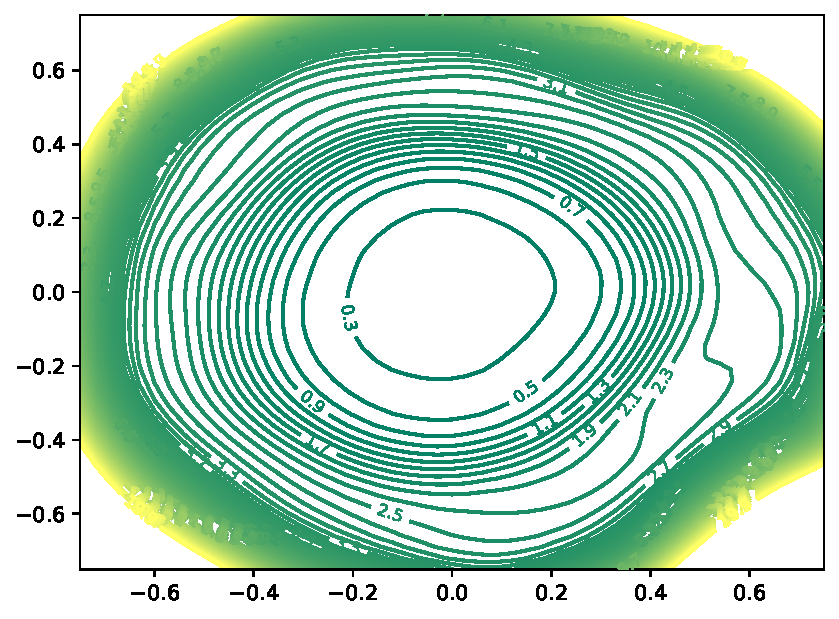
\includegraphics[width=.45\textwidth,height=!]{figs/075_51_test_loss_2dcontour.pdf} &
%     \hspace*{-5mm}  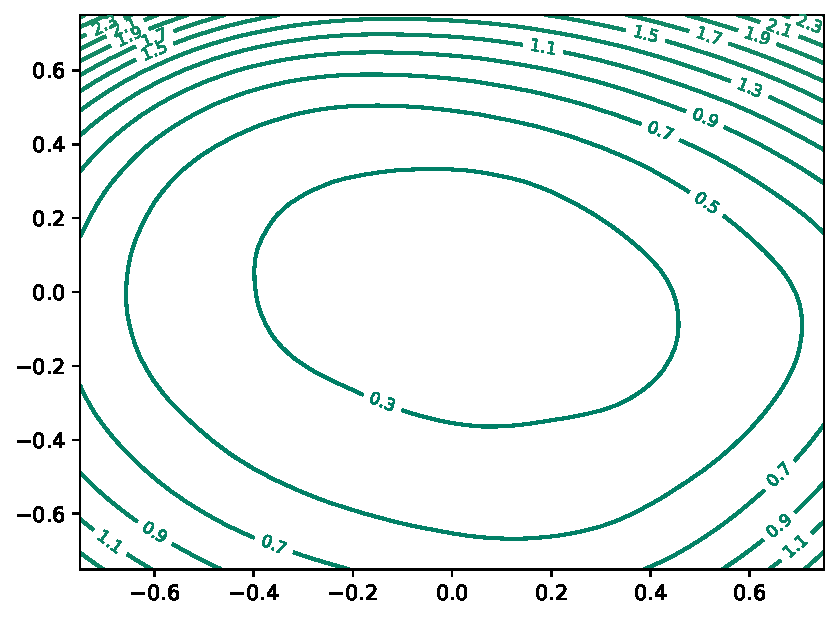
\includegraphics[width=.45\textwidth,height=!]{figs/075_51_sparse_test_loss_2dcontour.pdf} 
% \end{tabular}}
% % \vspace*{-3mm}
% \caption{\footnotesize{ Loss landscapes evaluated on the dense model (left) and the 95\%-sparse model (right) on the testing dataset of CIFAR-10. The x-axis and y-axis correspond to $\alpha$ and $\beta$ in \eqref{eq:losslandscape}, respectively.
% %the test dataset. \textbf{(Left)}: Dense model. \textbf{(Right)}: $95\%$ sparsity model.
% }}
% % \vspace*{-3mm}
% \label{fig: singular_sparsity}
% \end{figure}

\noindent \textbf{Model sparsity benefits privacy of {\MU} for `free'.}
It was  recently shown in \cite{huang2020privacy,wang2020against} that model sparsification helps protect data privacy, in terms of defense against MIA  used to infer training data  information   from a learned model. Inspired by the above, we ask if sparsity can also bring  the privacy benefit to an unlearned model, evaluated by  the MIA rate on the remaining dataset $\Dr$ (that we term \textbf{\MIAR}).  This is different from  {\MIAF}, which
reflects the efficacy of scrubbing ${\Df}$, \textit{i.e.}, correctly predicting that    data sample in ${\Df}$ is not in the training set of the unlearned model. In contrast, 
%similar to the definition of {\MIAF}. Yet, 
%It is also worth noting that one can similarly define {\MIAR}, given by   the MIA rate on the retaining dataset $\Dr$.  However, 
%Different from {\MIAF},
{\MIAR}  characterizes the   \textit{privacy}   of the unlearned model about $\Dr$. A \textit{lower} {\MIAR}   implies \textit{less} information leakage.


% \JH{Should we remove this part? we can put them in the appendix.}

\begin{wrapfigure}{r}{40mm}
%\vspace*{-4.2mm}
\centerline{
% \hspace*{-3mm}
%\begin{tabular}{cc}
%\hspace*{0mm}\includegraphics[width=.3\textwidth,height=!]{figure/performance_comparison.pdf}  
%&
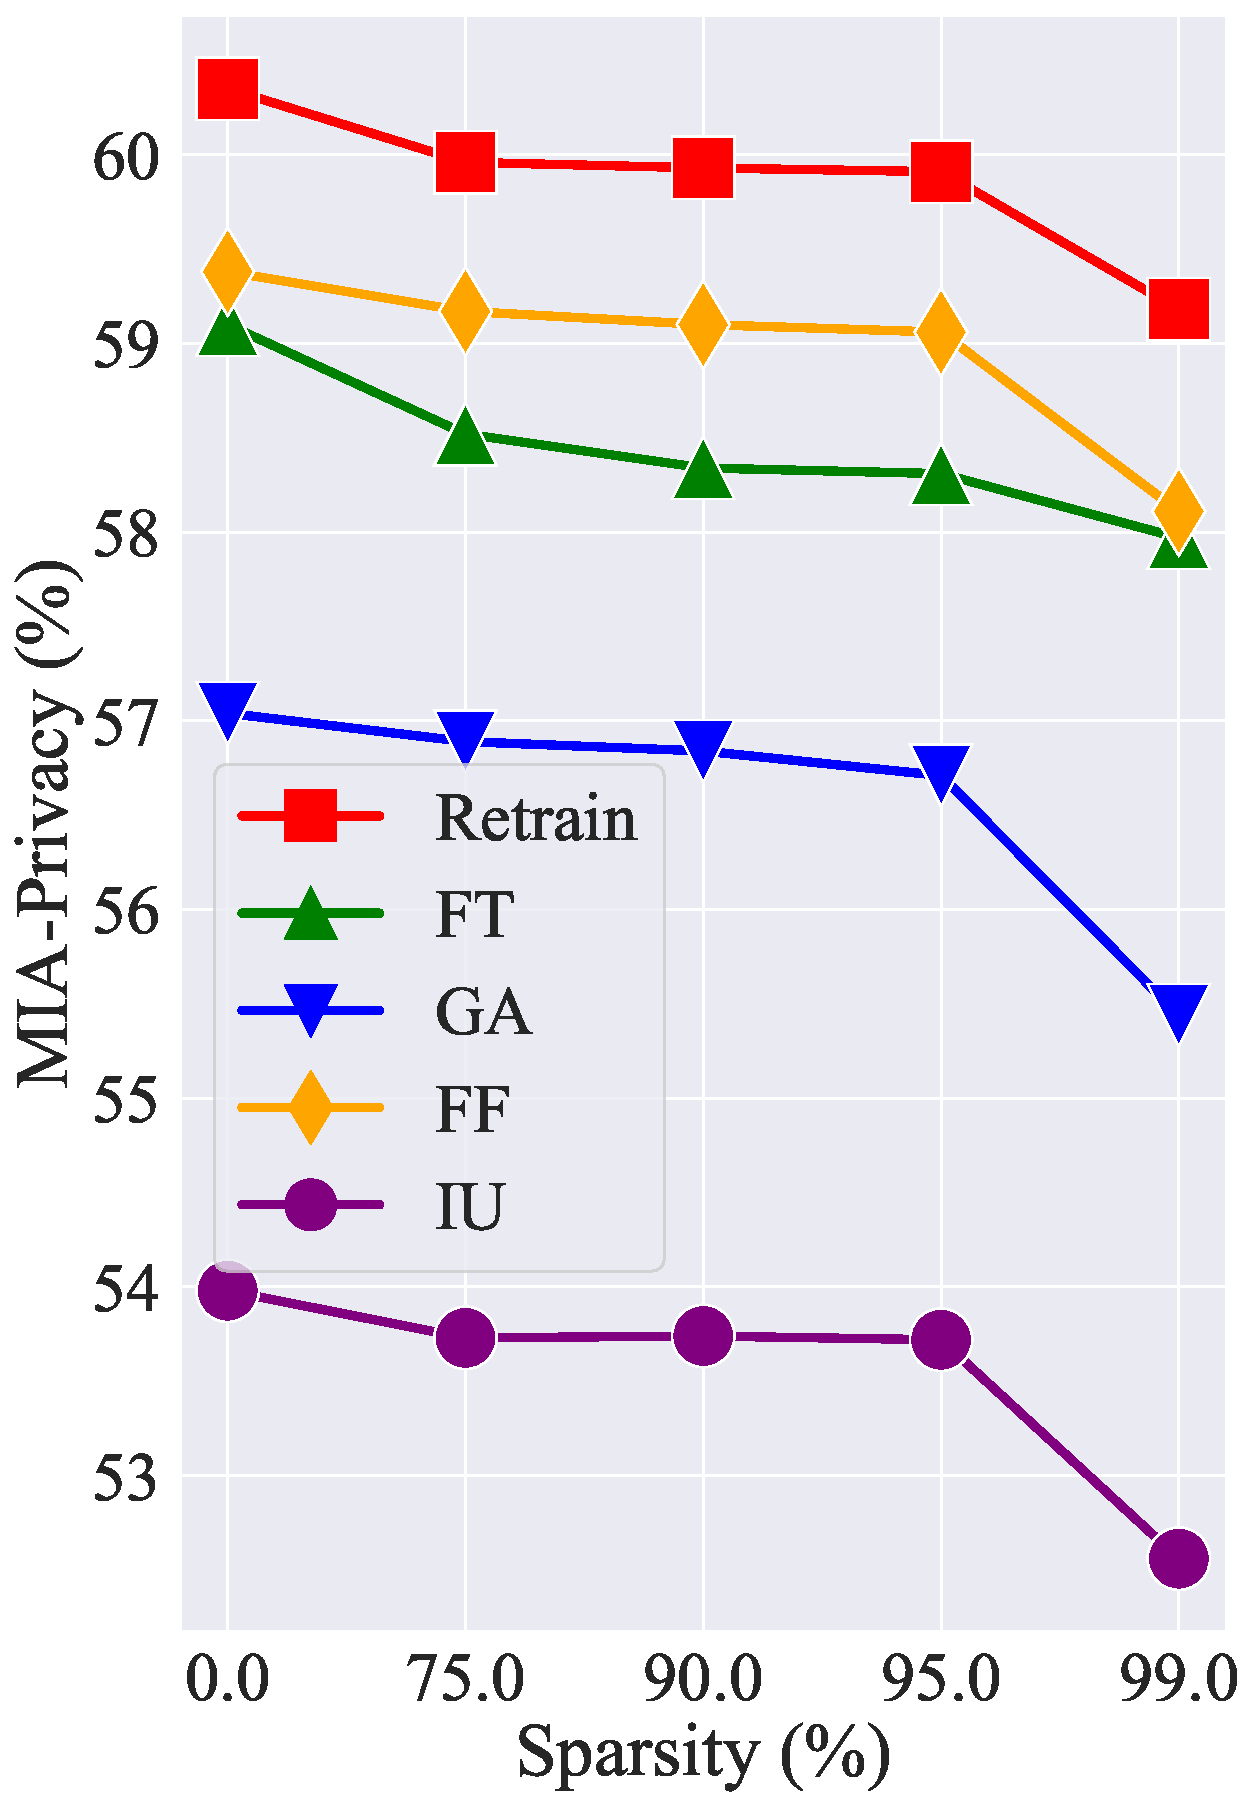
\includegraphics[width=40mm]{figs/privacy.pdf}
% \\
% \hspace*{2mm}\footnotesize{(a) Test accuracy vs. pruning ratio.} &   \footnotesize{(b) Runtime of pruning.}
%\end{tabular}
}
\vspace*{-1.5mm}
\caption{\footnotesize{Privacy on $\Dr$ ({\MIAR}) using different unlearning methods vs. model sparsity.
%\SL{[please use wrapfigure.]}
%[retrain,fisher,FT, GA, IU]
}}
  \label{fig: results_privacy}
\vspace*{-6.5mm}
  
\end{wrapfigure}
\textbf{Fig.\,\ref{fig: results_privacy}} shows {\MIAR} of
unlearned models versus the   sparsity ratio applied to different   unlearning methods in the `prune first, then unlearn' paradigm. 
As we can see, 
{\MIAR} decreases as the sparsity   increases. This suggests the improved  privacy 
of  unlearning on sparse models.
Moreover, we observe that approximate unlearning outperforms exact unlearning ({\retrain}) in   privacy preservation of $\Dr$. This is because {\retrain}  is conducted over ${\Dr}$ from scratch, leading to the strongest dependence on ${\Dr}$ than other unlearning methods.  Another interesting observation is that {\IU} and {\GA} yield a much smaller  {\MIAR}  than other approximate unlearning methods. The rationale behind that is   {\IU} and {\GA} have a weaker correlation with ${\Dr}$ during unlearning. Specifically,  the unlearning loss of {\IU}  only involves the forgetting data influence weights, \textit{i.e.}, $(\mathbf 1/N - \mathbf w)$ in \eqref{eq: Delta_IU}.
%although  {\IU}  calls for the Hessian and gradient information of the pre-trained original model. 
Similarly, {\GA} only performs gradient ascent   over $\Df$, with the least dependence on $\Dr$.  




\noindent \textbf{Performance of `prune first, then unlearn' on various datasets and architectures.}
\iffalse
In Tab.\,\ref{tab: overall_performance_ext_datasets} and Tab.\,\ref{tab: overall_performance_ext_archs}, we show that sparsity can reduce the performance gap between approximate unlearning and exact unlearning on various datasets and architectures (VGG-16) in different unlearning scenarios.
% and different model architectures in the class-wise forgetting unlearning scenario.
As we can see, model sparsity improves {\UA} and {\MIAF} without much performance loss in {\RA} and {\TA} across different settings in different unlearning scenarios, which is consistent with results shown in Tab.\,\ref{tab: overall_performance}. 
\fi
As demonstrated in Tab.\,\ref{tab: overall_performance_ext_datasets} and Tab.\,\ref{tab: overall_performance_ext_archs}, the introduction of model sparsity can effectively reduce the discrepancy between approximate and exact unlearning across a diverse range of datasets and architectures. This phenomenon is observable in various unlearning scenarios. Remarkably, model sparsity enhances both {\UA} and {\MIAF} metrics without incurring substantial degradation on {\RA} and {\TA} in different unlearning scenarios. These observations corroborate the findings reported in Tab.\,\ref{tab: overall_performance}. 
%\JC{[updated.]}

\begin{table*}[htb]
\centering
\caption{MU  performance vs. sparsity on additional datasets (CIFAR-100 \cite{krizhevsky2009learning} and SVHN \cite{netzer2011reading}) for both class-wise forgetting and random data forgetting. The content format follows Tab.\,\ref{tab: overall_performance}.
%\JC{[updated.]}
%\JC{[update caption]}
}
\label{tab: overall_performance_ext_datasets}
\resizebox{0.95\textwidth}{!}{
\begin{tabular}{c|cc|cc|cc|cc|c}
\toprule[1pt]
\midrule
  \multirow{2}{*}{\MU}& \multicolumn{2}{c|}{{\UA}} & \multicolumn{2}{c|}{{\MIAF}}& \multicolumn{2}{c|}{{\RA}} & \multicolumn{2}{c|}{{\TA}}&{\RTE}  \\ 
  & \multicolumn{1}{c|}{{\textsc{Dense}}}  & \multicolumn{1}{c|}{$\mathbf{95\%}$ \textbf{Sparsity}}
    & \multicolumn{1}{c|}{\textsc{Dense}}  & \multicolumn{1}{c|}{$\mathbf{95\%}$ \textbf{Sparsity}}
    & \multicolumn{1}{c|}{\textsc{Dense}}  & \multicolumn{1}{c|}{$\mathbf{95\%}$ \textbf{Sparsity}}
      & \multicolumn{1}{c|}{\textsc{Dense}}  & \multicolumn{1}{c|}{$\mathbf{95\%}$ \textbf{Sparsity}} & (min)
  \\
% \cline{3-10}

\midrule
\rowcolor{Gray}
\multicolumn{10}{c}{Class-wise forgetting, CIFAR-100} \\
\midrule
 \retrain &\textcolor{blue}{$100.00_{\pm{0.00}}$}   & \textcolor{blue}{$100.00_{\pm{0.00}}$} 
  &\textcolor{blue}{$100.00_{\pm{0.00}}$}   & \textcolor{blue}{$100.00_{\pm{0.00}}$}
   &\textcolor{blue}{$99.97_{\pm{0.01}}$}   & \textcolor{blue}{$96.68_{\pm{0.15}}$}
   &\textcolor{blue}{$73.74_{\pm{0.19}}$}   & \textcolor{blue}{$69.49_{\pm{0.41}}$} 
& $48.45$
 \\
 \FT &$15.00_{\pm{4.86}}$ (\textcolor{blue}{$85.00$})      & ${46.39}_{\pm{5.59}}$ (\textcolor{blue}{$53.61$}) 
  &$66.11_{\pm{4.53}}$ (\textcolor{blue}{$33.89$})    & ${67.17}_{\pm{5.91}}$ (\textcolor{blue}{$32.83$}) 
   &$99.87_{\pm{0.05}}$(\textcolor{blue}{$0.10$})   & $97.78_{\pm{0.52}}$ (\textcolor{blue}{$1.10$}) 
   &$74.88_{\pm{0.18}}$ (\textcolor{blue}{$1.14$}) &  ${72.53}_{\pm{0.11}}$ (\textcolor{blue}{$3.04$}) &$1.90$
 \\
 \GA  &$81.47_{\pm{0.32}}$(\textcolor{blue}{$18.53$})   & ${99.01}_{\pm{0.01}}$ (\textcolor{blue}{$0.99$}) 
 & $93.47_{\pm{4.56}}$ (\textcolor{blue}{$6.53$})  &${100.00}_{\pm{0.00}}$ (\textcolor{blue}{$0.00$}) 
 & $90.33_{\pm{1.71}}$ (\textcolor{blue}{$9.64$}) &$80.45_{\pm{0.78}}$ (\textcolor{blue}{$16.23$}) 
 & $64.94_{\pm{0.74}}$ (\textcolor{blue}{$8.80$})  & $60.99_{\pm{0.14}}$ (\textcolor{blue}{$8.50$})  
& $0.21$
 \\
 % \FF & \\
\IU &$84.12_{\pm{0.34}}$ (\textcolor{blue}{$15.88$}) &${99.78}_{\pm{0.01}}$ (\textcolor{blue}{$0.22$}) 
& $98.44_{\pm{0.45}}$ (\textcolor{blue}{$1.56$}) &${99.33}_{\pm{0.00}}$  (\textcolor{blue}{$0.67$}) 
& $96.23_{\pm{0.02}}$ (\textcolor{blue}{$3.74$}) & $95.45_{\pm{0.17}}$ (\textcolor{blue}{$1.23$}) 
&$71.24_{\pm{0.22}}$ (\textcolor{blue}{$2.50$}) & ${70.79}_{\pm{0.11}}$ (\textcolor{blue}{$0.95$}) 
& $4.30$
\\
% \FTSparse & 
% $94.55_{\pm{2.82}}$& $97.02_{\pm{2.60}}$ & $88.06_{\pm{3.14}}$&$63.61_{\pm2.25}$
% $94.55_{\pm{2.82}}$& $97.02_{\pm{2.60}}$ & $88.06_{\pm{3.14}}$&$63.61_{\pm2.25}$
% & -&-  & -&-
% \\
% \FTAO   & -&-  & -&-
% &$65.82_{\pm{12.66}}$ & $86.18_{\pm{7.08}}$ & $98.79_{\pm{0.21}}$&$73.54_{\pm0.08}$
% &$74.27_{\pm{5.34}}$& $93.42_{\pm{2.82}}$&  $97.70_{\pm{0.21}}$ &$72.54_{\pm0.32}$
% \\
\midrule
\rowcolor{Gray}
\multicolumn{10}{c}{Random data forgetting, CIFAR-100} \\
\midrule
 \retrain &\textcolor{blue}{$24.76_{\pm{0.12}}$}   & \textcolor{blue}{$27.64_{\pm{1.03}}$} 
  &\textcolor{blue}{$49.80_{\pm{0.26}}$}   & \textcolor{blue}{$44.87_{\pm{0.81}}$}
   &\textcolor{blue}{$99.98_{\pm{0.02}}$}   & \textcolor{blue}{$99.24_{\pm{0.02}}$}
   &\textcolor{blue}{$74.46_{\pm{0.08}}$}   & \textcolor{blue}{$69.78_{\pm{0.15}}$} 
& $48.70$
 \\
 % \FT & $0.78_{\pm{0.34}}$ (\textcolor{blue}{$23.98$})& $1.13_{\pm{0.40}}$ (\textcolor{blue}{$48.67$})& $99.93_{\pm{0.02}}$ (\textcolor{blue}{$0.05$})& $75.14_{\pm{0.09}}$ (\textcolor{blue}{$0.68$}) & 3.74 
 
 \FT &$0.78_{\pm{0.34}}$ (\textcolor{blue}{$23.98$})    & ${8.37}_{\pm{1.63}}$ (\textcolor{blue}{$19.27$}) 
  & $11.13_{\pm{0.40}}$ (\textcolor{blue}{$38.67$})   & ${18.57}_{\pm{1.57}}$ (\textcolor{blue}{$26.30$}) 
   &$99.93_{\pm{0.02}}$ (\textcolor{blue}{$0.05$})   & $99.20_{\pm{0.27}}$ (\textcolor{blue}{$0.04$}) 
   &$75.14_{\pm{0.09}}$ (\textcolor{blue}{$0.68$}) &  ${73.18}_{\pm{0.30}}$ (\textcolor{blue}{$1.60$}) &$3.74$
 \\
 \GA  &$0.04_{\pm{0.02}}$(\textcolor{blue}{$24.75$})   & ${3.92}_{\pm{0.28}}$ (\textcolor{blue}{$23.72$}) 
 & $3.80_{\pm{0.87}}$ (\textcolor{blue}{$46.00$})  &${7.51}_{\pm{1.37}}$ (\textcolor{blue}{$37.36$}) 
 & $99.97_{\pm{0.01}}$ (\textcolor{blue}{$0.01$}) &$98.40_{\pm{1.22}}$ (\textcolor{blue}{$0.84$}) 
 & $74.07_{\pm{0.11}}$ (\textcolor{blue}{$0.39$})  & $72.19_{\pm{0.15}}$ (\textcolor{blue}{$2.41$})  
& $0.24$
 \\
 % \FF & \\
\IU &$1.53_{\pm{0.36}}$ (\textcolor{blue}{$23.23$}) &${6.01}_{\pm{0.17}}$ (\textcolor{blue}{$21.63$}) 
& $6.58_{\pm{0.42}}$ (\textcolor{blue}{$43.22$}) &${11.47}_{\pm{0.54}}$  (\textcolor{blue}{$33.40$}) 
& $99.01_{\pm{0.28}}$ (\textcolor{blue}{$0.97$}) & $96.53_{\pm{0.24}}$ (\textcolor{blue}{$2.71$}) 
&$71.76_{\pm{0.31}}$ (\textcolor{blue}{$2.70$}) & ${69.40}_{\pm{0.19}}$ (\textcolor{blue}{$0.38$}) 
& $3.80$
\\
% \FTSparse & 
% $94.55_{\pm{2.82}}$& $97.02_{\pm{2.60}}$ & $88.06_{\pm{3.14}}$&$63.61_{\pm2.25}$
% $94.55_{\pm{2.82}}$& $97.02_{\pm{2.60}}$ & $88.06_{\pm{3.14}}$&$63.61_{\pm2.25}$
% & -&-  & -&-
% \\
% \FTAO   & -&-  & -&-
% &$65.82_{\pm{12.66}}$ & $86.18_{\pm{7.08}}$ & $98.79_{\pm{0.21}}$&$73.54_{\pm0.08}$
% &$74.27_{\pm{5.34}}$& $93.42_{\pm{2.82}}$&  $97.70_{\pm{0.21}}$ &$72.54_{\pm0.32}$
% \\
\midrule
\rowcolor{Gray}
\multicolumn{10}{c}{Class-wise forgetting, SVHN} \\
\midrule
 \retrain &\textcolor{blue}{$100.00_{\pm{0.00}}$}  & \textcolor{blue}{$100.00_{\pm{0.00}}$} 
 & \textcolor{blue}{$100.00_{\pm{0.00}}$}&  \textcolor{blue}{$100.00_{\pm{0.00}}$ }
& \textcolor{blue}{$100.00_{\pm{0.00}}$} &  \textcolor{blue}{$100.00_{\pm{0.00}}$}  
 &  \textcolor{blue}{$95.71_{\pm{0.12}}$}& \textcolor{blue}{$94.95_{\pm{0.05}}$ } & $42.84$
 \\
 \FT & {$11.48_{\pm{8.12}}$ } (\textcolor{blue}{$88.52$})    & ${51.93}_{\pm{19.62}}$ (\textcolor{blue}{$48.07$}) 
& $86.12_{\pm{9.62}}$ (\textcolor{blue}{$13.88$}) &${99.42}_{\pm{0.51}}$  (\textcolor{blue}{$0.58$}) 
& $100.00_{\pm{0.00}}$ (\textcolor{blue}{$0.00$}) &  $99.00_{\pm{0.00}}$ (\textcolor{blue}{$1.00$}) 
& $95.99_{\pm{0.07}}$ (\textcolor{blue}{$0.28$})&  $95.89_{\pm{0.02}}$ (\textcolor{blue}{$0.94$}) & $2.86$
 \\
  \GA &$83.87_{\pm{0.19}}$ (\textcolor{blue}{$16.13$})   & ${86.52}_{\pm{0.11}}$ (\textcolor{blue}{$13.48$}) 
  & $99.97_{\pm{0.02}}$ (\textcolor{blue}{$0.03$})&  ${100.00}_{\pm{0.00}}$ (\textcolor{blue}{$0.00$}) 
  & $99.60_{\pm{0.15}}$ (\textcolor{blue}{$0.40$})&$98.37_{\pm{0.11}}$ (\textcolor{blue}{$1.63$})  
  &  $95.27_{\pm{0.02}}$ (\textcolor{blue}{$0.44$})& $93.42_{\pm{0.07}}$ (\textcolor{blue}{$1.53$}) & $0.28$
  
  \\
% \FF & & & & & & & & &   \\
\IU &$95.11_{\pm{0.02}}$ (\textcolor{blue}{$4.89$})   & ${100.00}_{\pm{0.00}}$ (\textcolor{blue}{$0.00$}) 
&$99.89_{\pm{0.04}}$ (\textcolor{blue}{$0.11$})  & ${100.00}_{\pm{0.00}}$(\textcolor{blue}{$0.00$}) 
&$100.00_{\pm{0.00}}$ (\textcolor{blue}{$0.00$})   & $99.85_{\pm{0.02}}$ (\textcolor{blue}{$0.15$}) 
&$95.70_{\pm{0.09}}$ (\textcolor{blue}{$0.01$})   & $94.90_{\pm{0.04}}$ (\textcolor{blue}{$0.05$}) & $3.19$
\\
\midrule
\rowcolor{Gray}
\multicolumn{10}{c}{Random data forgetting, SVHN} \\
\midrule
 \retrain &\textcolor{blue}{$4.89_{\pm{0.11}}$}&\textcolor{blue}{$ 4.78_{\pm{0.23}}$}&\textcolor{blue}{$15.38_{\pm{0.14}}$}&\textcolor{blue}{$15.25_{\pm{0.18}}$}&\textcolor{blue}{$100.00_{\pm{0.00}}$}&\textcolor{blue}{$100.00_{\pm{0.00}}$}&\textcolor{blue}{$95.54_{\pm{0.09}}$}&\textcolor{blue}{$95.44_{\pm{0.12}}$} & 42.71
\\
 \FT & $2.28_{\pm{1.41}}$ (\textcolor{blue}{$2.61$})& $3.77_{\pm{0.13}}$ (\textcolor{blue}{$1.01$})& $6.14_{\pm{3.30}}$ (\textcolor{blue}{$9.24$})& $8.38_{\pm{0.42}}$ (\textcolor{blue}{$6.87$})& $99.71_{\pm{0.33}}$ (\textcolor{blue}{$0.29$})& $99.31_{\pm{0.33}}$ (\textcolor{blue}{$0.69$})& $94.77_{\pm{0.87}}$ (\textcolor{blue}{$0.77$})& $93.92_{\pm{0.34}}$ (\textcolor{blue}{$1.52$}) & 2.73
 \\
 \GA & $0.99_{\pm{0.42}}$ (\textcolor{blue}{$3.90$})& $2.68_{\pm{0.53}}$ (\textcolor{blue}{$2.10$})& $3.07_{\pm{0.53}}$ (\textcolor{blue}{$12.31$})& $9.31_{\pm{0.48}}$ (\textcolor{blue}{$5.94$})& $99.43_{\pm{0.22}}$ (\textcolor{blue}{$0.57$})& $97.83_{\pm{0.43}}$ (\textcolor{blue}{$2.17$})& $94.03_{\pm{0.21}}$ (\textcolor{blue}{$1.51$})& $93.33_{\pm{0.27}}$ (\textcolor{blue}{$2.11$}) & 0.26

  \\
% \FF & & & & & & & & &   \\
\IU &$3.48_{\pm{0.13}}$ (\textcolor{blue}{$1.41$})   & ${5.62}_{\pm{0.48}}$ (\textcolor{blue}{$0.84$}) 
&$9.44_{\pm{0.27}}$ (\textcolor{blue}{$5.94$})  & ${12.28}_{\pm{0.41}}$(\textcolor{blue}{$2.97$}) 
&$96.30_{\pm{0.08}}$ (\textcolor{blue}{$3.70$})   & $95.67_{\pm{0.15}}$ (\textcolor{blue}{$4.33$}) 
&$91.59_{\pm{0.11}}$ (\textcolor{blue}{$3.95$})   & $90.91_{\pm{0.26}}$ (\textcolor{blue}{$4.53$}) & $3.21$
\\
\midrule
\bottomrule[1pt]
\end{tabular}
}

\end{table*}
% \SL{[what is this table ???]}




% \begin{table*}[h]
% \centering
% \caption{\footnotesize{Performance overview of MU VS. Sparsity on different datasets, where the content format follows Table\,\ref{tab: overall_performance}.}}
% \label{tab: overall_performance_ext_datasets}
% \resizebox{0.95\textwidth}{!}{
% \begin{tabular}{c|ccc|ccc|ccc|ccc|c}
% \toprule[1pt]
% \midrule
%   \multirow{2}{*}{\MU}& \multicolumn{3}{c|}{{\UA}} & \multicolumn{3}{c|}{{\MIAF}}& \multicolumn{3}{c|}{{\RA}} & \multicolumn{3}{c|}{{\TA}}&\multirow{2}{*}{\RTE}  \\ 
%   & \multicolumn{1}{c|}{\textsc{Dense}} & \multicolumn{1}{c|}{$75\%$} & \multicolumn{1}{c|}{$95\%$}
%     & \multicolumn{1}{c|}{\textsc{Dense}} & \multicolumn{1}{c|}{$75\%$} & \multicolumn{1}{c|}{$95\%$}
%     & \multicolumn{1}{c|}{\textsc{Dense}} & \multicolumn{1}{c|}{$75\%$} & \multicolumn{1}{c|}{$95\%$}
%       & \multicolumn{1}{c|}{\textsc{Dense}} &  \multicolumn{1}{c|}{$75\%$} & \multicolumn{1}{c|}{$95\%$}
%   \\
% % \cline{3-10}

% \midrule
% \rowcolor{Gray}
% \multicolumn{14}{c}{\Large Cifar100} \\
% \midrule
%  \retrain &\textcolor{blue}{$100.00_{\pm{0.00}}$}  &  \textcolor{blue}{$100.00_{\pm{0.00}}$} & \textcolor{blue}{$100.00_{\pm{0.00}}$} 
%   &\textcolor{blue}{$100.00_{\pm{0.00}}$}  &  \textcolor{blue}{$100.00_{\pm{0.00}}$} & \textcolor{blue}{$100.00_{\pm{0.00}}$}
%    &\textcolor{blue}{$99.97_{\pm{0.01}}$}  &  \textcolor{blue}{$99.96_{\pm{0.01}}$} & \textcolor{blue}{$96.68_{\pm{0.15}}$}
%    &\textcolor{blue}{$73.74_{\pm{0.19}}$}  & \textcolor{blue}{ $73.23_{\pm{0.17}}$} & \textcolor{blue}{$69.49_{\pm{0.41}}$} 
% & 
%  \\
%  \FT &$14.80_{\pm{6.29}}$ ({\textcolor{blue}{$\LARGE\downarrow$}}85.20)    &  $17.20_{\pm{5.50}}$ ({\textcolor{blue}{$\LARGE\downarrow$}}82.80)  & $\mathbf{42.22}_{\pm{5.06}}$ ({\textcolor{blue}{$\LARGE\downarrow$}}57.78) 
%   &$69.82_{\pm{5.93}}$ ({\textcolor{blue}{$\LARGE\downarrow$}}30.18)  &  $72.40_{\pm{9.98}}$ ({\textcolor{blue}{$\LARGE\downarrow$}}27.60)  & $\mathbf{84.40}_{\pm{4.32}}$ ({\textcolor{blue}{$\LARGE\downarrow$}}15.60) 
%    &$99.86_{\pm{0.04}}$({\textcolor{blue}{$\LARGE\downarrow$}}0.14)   &  $99.87_{\pm{0.05}}$  ({\textcolor{blue}{$\LARGE\downarrow$}}0.13) & $97.72_{\pm{0.47}}$ ({\textcolor{blue}{$\LARGE\downarrow$}}2.28) 
%    &$72.16_{\pm{0.22}}$ ({\textcolor{blue}{$\LARGE\downarrow$}}1.58)   &  $72.28_{\pm{0.13}}$ ({\textcolor{blue}{$\LARGE\downarrow$}}0.95)  & $\mathbf{70.44}_{\pm{0.11}}$ ({\textcolor{blue}{$\LARGE\uparrow$}}0.95) 
%  \\
%  \GA  &$81.47_{\pm{0.32}}$({\textcolor{blue}{$\LARGE\downarrow$}}18.53)  &$87.38_{\pm{0.41}}$ ({\textcolor{blue}{$\LARGE\downarrow$}}12.62)  & $\mathbf{99.01}_{\pm{0.01}}$ ({\textcolor{blue}{$\LARGE\downarrow$}}0.99) 
%  & $93.47_{\pm{4.56}}$ ({\textcolor{blue}{$\LARGE\downarrow$}}6.53)  &$97.42_{\pm{0.11}}$ ({\textcolor{blue}{$\LARGE\downarrow$}}2.58) &$\mathbf{100.00}_{\pm{0.00}}$ ({\textcolor{blue}{$\LARGE\downarrow$}}0.00) 
%  & $90.33_{\pm{1.71}}$ ({\textcolor{blue}{$\LARGE\downarrow$}}9.64) & $91.27_{\pm{1.02}}$ ({\textcolor{blue}{$\LARGE\downarrow$}}8.69) &$80.45_{\pm{0.78}}$ ({\textcolor{blue}{$\LARGE\downarrow$}}16.23) 
%  & $64.94_{\pm{0.74}}$ ({\textcolor{blue}{$\LARGE\downarrow$}}8.80) &$65.36_{\pm{0.21}}$ ({\textcolor{blue}{$\LARGE\downarrow$}}7.86) & $60.99_{\pm{0.14}}$ ({\textcolor{blue}{$\LARGE\downarrow$}}8.50)  
% &
%  \\
%  % \FF & \\
% \IU &$98.00_{\pm{0.34}}$ ({\textcolor{blue}{$\LARGE\downarrow$}}2.00)  &$97.88_{\pm{0.21}}$ ({\textcolor{blue}{$\LARGE\downarrow$}}2.22) &$\mathbf{99.78}_{\pm{0.01}}$ ({\textcolor{blue}{$\LARGE\downarrow$}}0.22) 
% & $100.00_{\pm{0.00}}$ ({\textcolor{blue}{$\LARGE\downarrow$}}0.00)  & $100.00_{\pm{0.00}}$ ({\textcolor{blue}{$\LARGE\downarrow$}}0.00)  &$\mathbf{100.00}_{\pm{0.00}}$  ({\textcolor{blue}{$\LARGE\downarrow$}}0.00) 
% & $99.43_{\pm{0.02}}$ ({\textcolor{blue}{$\LARGE\downarrow$}}0.54) &$99.60_{\pm{1.02}}$ ({\textcolor{blue}{$\LARGE\downarrow$}}0.30) & $97.68_{\pm{0.17}}$ ({\textcolor{blue}{$\LARGE\uparrow$}}1.00) 
% &$72.16_{\pm{0.22}}$ ({\textcolor{blue}{$\LARGE\downarrow$}}1.58) &$72.28_{\pm{0.13}}$ ({\textcolor{blue}{$\LARGE\downarrow$}}0.95) & $\mathbf{70.44}_{\pm{0.11}}$ ({\textcolor{blue}{$\LARGE\uparrow$}}0.95) 
% & 
% \\
% % \FTSparse & 
% % $94.55_{\pm{2.82}}$& $97.02_{\pm{2.60}}$ & $88.06_{\pm{3.14}}$&$63.61_{\pm2.25}$
% % $94.55_{\pm{2.82}}$& $97.02_{\pm{2.60}}$ & $88.06_{\pm{3.14}}$&$63.61_{\pm2.25}$
% % & -&-  & -&-
% % \\
% % \FTAO   & -&-  & -&-
% % &$65.82_{\pm{12.66}}$ & $86.18_{\pm{7.08}}$ & $98.79_{\pm{0.21}}$&$73.54_{\pm0.08}$
% % &$74.27_{\pm{5.34}}$& $93.42_{\pm{2.82}}$&  $97.70_{\pm{0.21}}$ &$72.54_{\pm0.32}$
% % \\
% \midrule
% \rowcolor{Gray}
% \multicolumn{14}{c}{\Large SVHN} \\
% \midrule
%  \retrain &\textcolor{blue}{$100.00_{\pm{0.00}}$}  &  \textcolor{blue}{$100.00_{\pm{0.00}}$} & \textcolor{blue}{$100.00_{\pm{0.00}}$} 
%  & \textcolor{blue}{$100.00_{\pm{0.00}}$} &\textcolor{blue}{$100.00_{\pm{0.00}}$}  &  \textcolor{blue}{$100.00_{\pm{0.00}}$ }
% & \textcolor{blue}{$100.00_{\pm{0.00}}$} &\textcolor{blue}{$100.00_{\pm{0.00}}$}  &  \textcolor{blue}{$100.00_{\pm{0.00}}$}  
%  &  \textcolor{blue}{$95.71_{\pm{0.12}}$} & \textcolor{blue}{$95.72_{\pm{0.12}}$} & \textcolor{blue}{$94.95_{\pm{0.05}}$ }
%  \\
%  \FT & {$11.48_{\pm{8.12}}$ } ({\textcolor{blue}{$\LARGE\downarrow$}}88.52)  &  $21.98_{\pm{14.87}}$ ({\textcolor{blue}{$\LARGE\downarrow$}}78.02)  & $\mathbf{51.93}_{\pm{19.62}}$ ({\textcolor{blue}{$\LARGE\downarrow$}}48.07) 
% & $86.12_{\pm{9.62}}$ ({\textcolor{blue}{$\LARGE\downarrow$}}13.88)  & $87.49_{\pm{8.93}}$ ({\textcolor{blue}{$\LARGE\downarrow$}}12.51) &$\mathbf{99.42}_{\pm{0.51}}$  ({\textcolor{blue}{$\LARGE\downarrow$}}0.58) 
% & $100.00_{\pm{0.00}}$ ({\textcolor{blue}{$\LARGE\downarrow$}}0.00)  &$100.00_{\pm{0.00}}$ ({\textcolor{blue}{$\LARGE\downarrow$}}0.00)  &  $99.00_{\pm{0.00}}$ ({\textcolor{blue}{$\LARGE\downarrow$}}1.00) 
% & $95.99_{\pm{0.07}}$ ({\textcolor{blue}{$\LARGE\uparrow$}}0.28) &$95.95_{\pm{0.09}}$  ({\textcolor{blue}{$\LARGE\uparrow$}}0.23) &  $95.89_{\pm{0.02}}$ ({\textcolor{blue}{$\LARGE\uparrow$}}0.94) 
%  \\
%   \GA &$83.87_{\pm{0.19}}$ ({\textcolor{blue}{$\LARGE\downarrow$}}16.33)   &  $84.89{\pm{0.12}}$ ({\textcolor{blue}{$\LARGE\downarrow$}}15.11) & $\mathbf{86.52}_{\pm{0.11}}$ ({\textcolor{blue}{$\LARGE\downarrow$}}13.48) 
%   & $99.97_{\pm{0.02}}$ ({\textcolor{blue}{$\LARGE\downarrow$}}0.03) &$100.00_{\pm{0.00}}$ ({\textcolor{blue}{$\LARGE\downarrow$}}0.00)  &  $\mathbf{100.00}_{\pm{0.00}}$ ({\textcolor{blue}{$\LARGE\downarrow$}}0.00) 
%   & $99.60_{\pm{0.15}}$ ({\textcolor{blue}{$\LARGE\downarrow$}}0.40) & $99.51_{\pm{0.13}}$ ({\textcolor{blue}{$\LARGE\downarrow$}}0.49) &$98.37_{\pm{0.11}}$ ({\textcolor{blue}{$\LARGE\downarrow$}}1.63)  
%   &  $95.27_{\pm{0.02}}$ ({\textcolor{blue}{$\LARGE\uparrow$}}0.44)  & $95.08_{\pm{0.01}}$({\textcolor{blue}{$\LARGE\downarrow$}}0.64)  & $93.42_{\pm{0.04}}$ ({\textcolor{blue}{$\LARGE\downarrow$}}1.53) 
  
%   \\
% % \FF & & & & & & & & &   \\
% \IU &$95.11_{\pm{0.02}}$ ({\textcolor{blue}{$\LARGE\downarrow$}}4.89)  &  $100.00_{\pm{0.00}}$ ({\textcolor{blue}{$\LARGE\downarrow$}}0.00) & $\mathbf{100.00}_{\pm{0.00}}$ ({\textcolor{blue}{$\LARGE\downarrow$}}0.00) 
% &$99.89_{\pm{0.04}}$ ({\textcolor{blue}{$\LARGE\downarrow$}}0.11  &  $100.00_{\pm{0.00}}$ ({\textcolor{blue}{$\LARGE\downarrow$}}0.00) & $\mathbf{100.00}_{\pm{0.00}}$({\textcolor{blue}{$\LARGE\downarrow$}}0.00) 
% &$100.00_{\pm{0.00}}$ ({\textcolor{blue}{$\LARGE\downarrow$}}0.00)  &  $99.99{\pm{0.01}}$ ({\textcolor{blue}{$\LARGE\downarrow$}}0.01)  & $99.85_{\pm{0.02}}$ ({\textcolor{blue}{$\LARGE\downarrow$}}0.15) 
% &$95.70_{\pm{0.07}}$ ({\textcolor{blue}{$\LARGE\downarrow$}}0.01)  &  $95.19_{\pm{0.04}}$ ({\textcolor{blue}{$\LARGE\downarrow$}}0.53)  & $94.90_{\pm{0.02}}$ ({\textcolor{blue}{$\LARGE\downarrow$}}0.05) 
% \\
% % \FTSparse & 
% % \\
% % \FTAO  & 
% % \\
% \midrule
% \rowcolor{Gray}
% \multicolumn{14}{c}{\Large TinyImagenet} \\
% \midrule
%  \retrain &\textcolor{blue}{$100.00_{\pm{0.00}}$}  &  \textcolor{blue}{$100.00_{\pm{0.00}}$} & \textcolor{blue}{$100.00_{\pm{0.00}}$} 
%  &\textcolor{blue}{$100.00_{\pm{0.00}}$}  & \textcolor{blue}{$100.00_{\pm{0.00}}$} & \textcolor{blue}{$100.00_{\pm{0.00}}$} 
%  &\textcolor{blue}{$99.98_{\pm{0.01}}$}  &  \textcolor{blue}{$99.98_{\pm{0.01}}$} & \textcolor{blue}{$90.89_{\pm{0.03}}$ }
%   &\textcolor{blue}{$65.01_{\pm{0.13}}$}  &  \textcolor{blue}{$62.56_{\pm{0.22}}$} & \textcolor{blue}{$58.46_{\pm{0.28}}$ }
%  \\
% \FT &$25.13_{\pm{1.20}}$ ({\textcolor{blue}{$\LARGE\downarrow$}}74.87)   &  $50.80_{\pm{2.59}}$ ({\textcolor{blue}{$\LARGE\downarrow$}}49.20) & $\mathbf{76.33}_{\pm{3.52}}$ ({\textcolor{blue}{$\LARGE\downarrow$}}23.67) 
% & $76.87_{\pm{0.47}}$ ({\textcolor{blue}{$\LARGE\downarrow$}}23.13)  &$87.07_{\pm{0.51}}$ ({\textcolor{blue}{$\LARGE\downarrow$}}12.93)  &  $\mathbf{97.13}_{\pm{0.68}}$ ({\textcolor{blue}{$\LARGE\downarrow$}}2.87) 
% & $99.98_{\pm{0.01}}$ ({\textcolor{blue}{$\LARGE\downarrow$}}0.00)  & $97.94_{\pm{0.05}}$ ({\textcolor{blue}{$\LARGE\downarrow$}}2.04) &$89.18_{\pm{0.40}}$  ({\textcolor{blue}{$\LARGE\downarrow$}}1.01) 
% &  $65.55_{\pm{0.18}}$({\textcolor{blue}{$\LARGE\uparrow$}}0.54)  & $64.27_{\pm{0.32}}$ ({\textcolor{blue}{$\LARGE\uparrow$}}1.27) & $59.74_{\pm{0.12}}$ ({\textcolor{blue}{$\LARGE\uparrow$}}1.28)   \\
% \GA &$83.87_{\pm{0.19}}$ ({\textcolor{blue}{$\LARGE\downarrow$}}16.17)  &  $86.67_{\pm{0.34}}$({\textcolor{blue}{$\LARGE\downarrow$}}13.33)  & $\mathbf{92.27}_{\pm{0.09}}$ ({\textcolor{blue}{$\LARGE\downarrow$}}7.73) 
%  &$90.20_{\pm{0.02}}$ ({\textcolor{blue}{$\LARGE\downarrow$}}9.80)  &  $92.87_{\pm{0.09}}$ ({\textcolor{blue}{$\LARGE\downarrow$}}7.13) & $\mathbf{97.00}_{\pm{0.04}}$ ({\textcolor{blue}{$\LARGE\downarrow$}}3.00) & $98.44_{\pm{0.01}}$ ({\textcolor{blue}{$\LARGE\downarrow$}}1.54)
%   &$85.16_{\pm{0.02}}$ ({\textcolor{blue}{$\LARGE\downarrow$}}14.82)  &  $80.78_{\pm{0.03}}$ ({\textcolor{blue}{$\LARGE\downarrow$}}10.11) & $59.84_{\pm{0.03}}$ ({\textcolor{blue}{$\LARGE\downarrow$}}5.17) & $58.68_{\pm{0.02}}$ ({\textcolor{blue}{$\LARGE\downarrow$}}3.88) & $\mathbf{55.74}_{\pm{0.03}}$ ({\textcolor{blue}{$\LARGE\downarrow$}}2.72) & \\
% % \FF & & & & & & & & &  \\
% \IU   &$89.60_{\pm{0.24}}$ ({\textcolor{blue}{$\LARGE\downarrow$}}16.17)  &  $94.00_{\pm{0.15}}$ ({\textcolor{blue}{$\LARGE\downarrow$}}6.00) & $\mathbf{95.81}_{\pm{0.07}}$ ({\textcolor{blue}{$\LARGE\downarrow$}}4.91)  

% &$100_{\pm{0.00}}$ ({\textcolor{blue}{$\LARGE\downarrow$}}0.00)  &  $100.00_{\pm{0.00}}$({\textcolor{blue}{$\LARGE\downarrow$}}0.00)  & $\mathbf{100.00}_{\pm{0.00}}$({\textcolor{blue}{$\LARGE\downarrow$}}0.00) 
% &$96.78_{\pm{0.03}}$ ({\textcolor{blue}{$\LARGE\downarrow$}}3.20)  &  $84.53_{\pm{0.21}}$ ({\textcolor{blue}{$\LARGE\downarrow$}}14.45)  & $82.11_{\pm{0.13}}$ ({\textcolor{blue}{$\LARGE\downarrow$}}8.78) 
% &$63.19_{\pm{0.05}}$ ({\textcolor{blue}{$\LARGE\downarrow$}}1.82)  &  $61.41_{\pm{0.01}}$ ({\textcolor{blue}{$\LARGE\downarrow$}}1.15)  & $58.73_{\pm{0.06}}$ ({\textcolor{blue}{$\LARGE\downarrow$}}0.26) 
% \\
% % \FTSparse & 
% % \\
% % \FTAO  & 
% % \\
% \midrule
% \bottomrule[1pt]
% \end{tabular}
% }
% \vspace*{-3mm}

% \end{table*}



\begin{table*}[htb]
\centering
\caption{MU performance vs. sparsity on the additional architecture (VGG-16 \cite{simonyan2014very}) for both class-wise forgetting and random data forgetting on CIFAR-10.  The content format follows Tab.\,\ref{tab: overall_performance}.
% \JC{[update caption and update random data forgetting]}
%\JC{[updated]}
}
\label{tab: overall_performance_ext_archs}
\resizebox{0.95\textwidth}{!}{
\begin{tabular}{c|cc|cc|cc|cc|c}
\toprule[1pt]
\midrule
  \multirow{2}{*}{\MU}& \multicolumn{2}{c|}{{\UA}} & \multicolumn{2}{c|}{{\MIAF}}& \multicolumn{2}{c|}{{\RA}} & \multicolumn{2}{c|}{{\TA}}&{\RTE}  \\ 
  & \multicolumn{1}{c|}{{\textsc{Dense}}}  & \multicolumn{1}{c|}{$\mathbf{95\%}$ \textbf{Sparsity}}
    & \multicolumn{1}{c|}{\textsc{Dense}}  & \multicolumn{1}{c|}{$\mathbf{95\%}$ \textbf{Sparsity}}
    & \multicolumn{1}{c|}{\textsc{Dense}}  & \multicolumn{1}{c|}{$\mathbf{95\%}$ \textbf{Sparsity}}
      & \multicolumn{1}{c|}{\textsc{Dense}}  & \multicolumn{1}{c|}{$\mathbf{95\%}$ \textbf{Sparsity}} & (min)
  \\
% \cline{3-10}

\midrule
\rowcolor{Gray}
\multicolumn{10}{c}{Class-wise forgetting, VGG-16} \\
\midrule
 \retrain &\textcolor{blue}{$100.00_{\pm{0.00}}$}   & \textcolor{blue}{$100.00_{\pm{0.00}}$} 
  &\textcolor{blue}{$100.00_{\pm{0.00}}$} &  \textcolor{blue}{$100.00_{\pm{0.00}}$}
   &\textcolor{blue}{$100.00_{\pm{0.01}}$}  & \textcolor{blue}{$99.97_{\pm{0.00}}$}
   &\textcolor{blue}{$94.83_{\pm{0.10}}$}   & \textcolor{blue}{$92.93_{\pm{0.06}}$} & $30.38$

 \\
 \FT &$28.00_{\pm{8.16}}$ (\textcolor{blue}{$72.00$})      & ${34.94}_{\pm{5.37}}$ (\textcolor{blue}{$65.06$}) 
  &$63.23_{\pm{17.68}}$ (\textcolor{blue}{$36.77$})    & ${68.02}_{\pm{12.03}}$ (\textcolor{blue}{$31.98$}) 
   &$99.87_{\pm{0.05}}$(\textcolor{blue}{$0.13$})    & $99.60_{\pm{0.08}}$ (\textcolor{blue}{$0.37$}) 
   &$92.80_{\pm{1.28}}$ (\textcolor{blue}{$2.03$})     & ${92.96}_{\pm{0.85}}$ (\textcolor{blue}{$0.03$}) & $1.81$
 \\
 \GA  &$77.51_{\pm{3.47}}$ (\textcolor{blue}{$22.49$})      & ${83.93}_{\pm{2.14}}$ (\textcolor{blue}{$16.07$}) 
  &$80.13_{\pm{4.27}}$ (\textcolor{blue}{$19.87$})    & ${88.04}_{\pm{3.18}}$ (\textcolor{blue}{$11.96$}) 
   &$96.09_{\pm{0.13}}$(\textcolor{blue}{$3.91$})    & ${97.33}_{\pm{0.08}}$ (\textcolor{blue}{$2.64$}) 
   &$88.80_{\pm{1.33}}$ (\textcolor{blue}{$6.03$})     & ${89.95}_{\pm{0.78}}$ (\textcolor{blue}{$2.98$}) & $0.27$
 \\
 % \FF & \\
\IU &$88.58_{\pm{0.86}}$ (\textcolor{blue}{$11.42$})      & ${98.78}_{\pm{0.44}}$ (\textcolor{blue}{$1.22$}) 
  &$92.27_{\pm{1.14}}$ (\textcolor{blue}{$7.73$})    & ${99.91}_{\pm{0.05}}$ (\textcolor{blue}{$0.09$}) 
   &$96.89_{\pm{0.27}}$(\textcolor{blue}{$3.11$})    & ${93.18}_{\pm{0.28}}$ (\textcolor{blue}{$6.79$}) 
   &$89.81_{\pm{1.01}}$ (\textcolor{blue}{$5.02$})     & ${87.45}_{\pm{0.81}}$ (\textcolor{blue}{$5.48$}) & $2.51$
\\


\midrule
\rowcolor{Gray}
\multicolumn{10}{c}{Random data forgetting, VGG-16} \\ %jjh nb ??? tiao canshu ne 
\midrule
 \retrain &\textcolor{blue}{$7.13_{\pm{0.60}}$}   & \textcolor{blue}{$7.47_{\pm{0.30}}$} 
  &\textcolor{blue}{$13.02_{\pm{0.77}}$} &  \textcolor{blue}{$13.51_{\pm{0.50}}$}
   &\textcolor{blue}{$100.00_{\pm{0.01}}$}  & \textcolor{blue}{$99.93_{\pm{0.01}}$}
   &\textcolor{blue}{$92.80_{\pm{0.17}}$}   & \textcolor{blue}{$91.98_{\pm{0.22}}$} & $30.29$

 \\
 \FT &$0.86_{\pm{0.29}}$ (\textcolor{blue}{$6.27$})      & ${1.46}_{\pm{0.22}}$ (\textcolor{blue}{$6.01$}) 
  &$2.62_{\pm{0.47}}$ (\textcolor{blue}{$10.40$})    & ${3.82}_{\pm{0.41}}$ (\textcolor{blue}{$9.69$}) 
   &$99.76_{\pm{0.12}}$(\textcolor{blue}{$0.24$})    & $99.47_{\pm{0.11}}$ (\textcolor{blue}{$0.53$}) 
   &$92.21_{\pm{0.13}}$ (\textcolor{blue}{$0.59$})     & ${92.03}_{\pm{0.37}}$ (\textcolor{blue}{$0.05$}) & $1.77$
 \\
 \GA & $9.11_{\pm{0.83}}$ (\textcolor{blue}{$1.98$})& $6.91_{\pm{0.96}}$ (\textcolor{blue}{$0.56$})& $7.77_{\pm{1.01}}$ (\textcolor{blue}{$5.25$})& $8.37_{\pm{1.35}}$ (\textcolor{blue}{$5.14$})& $93.08_{\pm{0.93}}$ (\textcolor{blue}{$6.92$})& $93.63_{\pm{1.16}}$ (\textcolor{blue}{$6.30$})& $86.44_{\pm{1.32}}$ (\textcolor{blue}{$6.36$})& $89.22_{\pm{1.59}}$ (\textcolor{blue}{$4.53$}) & 0.31
 \\
 % \FF & \\
\IU &$1.02_{\pm{0.43}}$ (\textcolor{blue}{$6.11$})      & ${3.07}_{\pm{0.50}}$ (\textcolor{blue}{$4.40$}) 
  &$2.51_{\pm{0.61}}$ (\textcolor{blue}{$9.51$})    & ${6.86}_{\pm{0.67}}$ (\textcolor{blue}{$6.65$}) 
   &$99.14_{\pm{0.03}}$(\textcolor{blue}{$0.86$})    & ${97.35}_{\pm{0.31}}$ (\textcolor{blue}{$2.58$}) 
   &$91.01_{\pm{0.29}}$ (\textcolor{blue}{$1.79$})     & ${89.49}_{\pm{0.37}}$ (\textcolor{blue}{$2.49$}) & $2.78$
\\
\midrule
\bottomrule[1pt]
\end{tabular}
}

\end{table*}




%\noindent \textbf{Overall performance on ImageNet.}
To demonstrate the effectiveness of our methods on a larger dataset, we conducted additional experiments on \textbf{ImageNet} \cite{deng2009imagenet} with settings consistent with the class-wise forgetting in Tab.\,\ref{tab: overall_performance}. 
As we can see from Tab.\,\ref{tab: overall_performance_ImageNet}, sparsity reduces the performance gap between exact unlearning (Retrain) and the   approximate unlearning methods (FT and GA). The results are consistent with our  observations in other datasets. Note that the $83\%$ model sparsity (ImageNet, ResNet-18) is used to preserve the TA performance after one-shot magnitude (OMP) pruning.

\begin{table*}[ht]
\centering
\caption{\footnotesize{Performance overview of MU vs. sparsity on ImageNet considering class-wise forgetting. The content format follows Tab.\,\ref{tab: overall_performance}.}}
\label{tab: overall_performance_ImageNet}
\resizebox{0.80\textwidth}{!}{
\begin{tabular}{c|cc|cc|cc|cc|c}
\toprule[1pt]
\midrule
  \multirow{2}{*}{\MU}& \multicolumn{2}{c|}{{\UA}} & \multicolumn{2}{c|}{{\MIAF}}& \multicolumn{2}{c|}{{\RA}} & \multicolumn{2}{c|}{{\TA}}&{\RTE}  \\ 
  & \multicolumn{1}{c|}{{\textsc{Dense}}}  & \multicolumn{1}{c|}{$\mathbf{83\%}$ \textbf{Sparsity}}
    & \multicolumn{1}{c|}{\textsc{Dense}}  & \multicolumn{1}{c|}{$\mathbf{83\%}$ \textbf{Sparsity}}
    & \multicolumn{1}{c|}{\textsc{Dense}}  & \multicolumn{1}{c|}{$\mathbf{83\%}$ \textbf{Sparsity}}
      & \multicolumn{1}{c|}{\textsc{Dense}}  & \multicolumn{1}{c|}{$\mathbf{83\%}$ \textbf{Sparsity}} & (hours)
  \\
% \cline{3-10}

\midrule
\rowcolor{Gray}
\multicolumn{10}{c}{Class-wise forgetting, ImageNet} \\
\midrule
 \retrain &\textcolor{blue}{$100.00$}&\textcolor{blue}{$100.00$}&\textcolor{blue}{$100.00$}&\textcolor{blue}{$100.00$}&\textcolor{blue}{$71.75$}&\textcolor{blue}{$69.18$}&\textcolor{blue}{$69.49$}&\textcolor{blue}{$68.86$} & 26.18
\\
 \FT & $63.60$ (\textcolor{blue}{$36.40$})& $74.66$ (\textcolor{blue}{$25.34$})& $68.61$ (\textcolor{blue}{$31.39$})& $81.43$ (\textcolor{blue}{$18.57$})& $72.45$ (\textcolor{blue}{$0.70$})& $69.36$ (\textcolor{blue}{$0.18$})& $69.80$ (\textcolor{blue}{$0.31$})& $68.77$ (\textcolor{blue}{$0.09$}) & 2.87
 \\
 \GA & $85.10$ (\textcolor{blue}{$14.90$})& $90.21$ (\textcolor{blue}{$9.79$})& $87.46$ (\textcolor{blue}{$12.54$})& $94.25$ (\textcolor{blue}{$5.75$})& $65.93$ (\textcolor{blue}{$5.82$})& $62.94$ (\textcolor{blue}{$6.24$})& $64.62$ (\textcolor{blue}{$4.87$})& $64.65$ (\textcolor{blue}{$4.21$}) & 0.01
 \\
\midrule
\bottomrule[1pt]
\end{tabular}
}
\end{table*}





\noindent \textbf{Performance of $\ell_1$ sparsity-aware {\MU} on additional datasets.}
\iffalse
As illustrated in Tab.\,\ref{tab: sparse_MU vs MU}, the employment of sparsity-aware {\MU} ({\MUSparse}) substantially reduces the disparity between the approximate and exact unlearning methods in diverse unlearning scenarios. This phenomenon is evident across multiple datasets, including CIFAR-10, CIFAR-100, SVHN, and ImageNet. 

In particular, {\MUSparse} demonstrates superior performance in both {\UA} and {\MIAF} metrics compared to other approaches. It achieves this while maintaining an acceptable level of performance in {\RA} and {\TA} metrics, making it a practical approach for many unlearning scenarios. For instance, in the case of class-wise forgetting, {\MUSparse}'s performance matches or closely approximates the performance of {\retrain}. Similarly, in the scenario of random data forgetting on CIFAR-10, {\MUSparse} achieves comparable results with {\retrain} method in terms of {\UA} and {\MIAF} metrics.

Another crucial observation is that the utilization of {\MUSparse} consistently improves the forgetting metrics while incurring a negligible amount of additional computational cost, represented by the {\RTE} metric. Across all evaluated scenarios, the increase in {\RTE} for {\MUSparse} compared to other approximate unlearning methods is minimal. These observations highlight the effectiveness and efficiency of sparsity-aware {\MU} in diverse unlearning scenarios, as depicted in Tab.\,\ref{tab: sparse_MU vs MU}.
\fi
As seen in Fig.\,\ref{fig: results_l1_sparse_unlearn_others},  {\MUSparse} significantly reduces the gap between approximate and exact unlearning methods across various datasets (CIFAR-100 \cite{krizhevsky2009learning}, SVHN \cite{netzer2011reading}, ImageNet \cite{deng2009imagenet}) in different unlearning scenarios. It notably outperforms other methods in {\UA} and {\MIAF} metrics while preserving acceptable {\RA} and {\TA} performances, thus becoming a practical choice for unlearning scenarios. In class-wise and random data forgetting cases, {\MUSparse} exhibits performance on par with {\retrain} in {\UA} and {\MIAF} metrics. Importantly, the use of {\MUSparse} consistently enhances forgetting metrics with an insignificant rise in computational cost compared with {\FT}, underscoring its effectiveness and efficiency in diverse unlearning scenarios. For detailed numerical results, please refer to Tab.\,\ref{tab: sparse_MU vs MU}. %\JC{[new.]}



\begin{figure*}[htb]
\centerline{
\begin{tabular}{ccccc}

\hspace{-1.2mm}
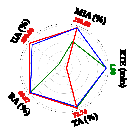
\includegraphics[width=25mm,height=!]{figs/cifar100_class_new-cropped.pdf}
\hspace{-1.2mm}
 & 
\hspace{-1.2mm}
 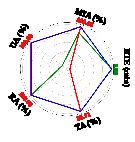
\includegraphics[width=25mm,height=!]{figs/svhn_class.pdf}
\hspace{-1.2mm}
& 
\hspace{-1.2mm}
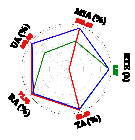
\includegraphics[width=25mm,height=!]{figs/imagenet_class.pdf}
\hspace{-1.2mm}
 & 
\hspace{-1.2mm}
 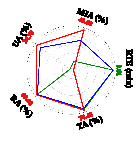
\includegraphics[width=25mm,height=!]{figs/cifar100_random_mew-cropped.pdf}
\hspace{-1.2mm}
 &
\hspace{-1.2mm}
 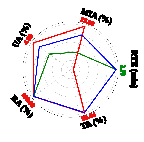
\includegraphics[width=25mm,height=!]{figs/svhn_random_new-cropped.pdf}
\hspace{-1.2mm}
% \vspace*{-2.5mm}
\\
% \multicolumn{4}{c}{\includegraphics[width=**]{figs/l1_sparse_legend.pdf}} \\
\scriptsize{CIFAR-100} & \scriptsize{SVHN} & \scriptsize{ImageNet} & \scriptsize{CIFAR-100} & \scriptsize{SVHN} \\
\scriptsize{Class-wise forgetting} & \scriptsize{Class-wise forgetting} & \scriptsize{Class-wise forgetting} & \scriptsize{Random data forgetting} & \scriptsize{Random data forgetting}
 \\
\multicolumn{5}{c}{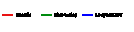
\includegraphics[width=50mm,height=!]{figs/legend.pdf}}\\
\end{tabular}}
\vspace*{-1.5mm}
\caption{
Performance   of sparsity-aware unlearning vs. {\FT} and {\retrain} on class-wise forgetting and random data forgetting under ResNet-18 on different datasets. 
 Each metric is normalized to $[0,1]$ based on the best result  across unlearning methods for ease of visualization, while the actual best value is provided. The figure format is consistent with Fig.\,\ref{fig: results_l1_sparse_unlearn}.
%\JC{[Should we mention Fig.\,\ref{fig: results_l1_sparse_unlearn}?]}
% \JC{[FIXME: The radar charts are still not aligned. @Jinghan]}
% \JH{[updated]}
}
%\JC{move other datasets (except cifar10) to appendix}
  \label{fig: results_l1_sparse_unlearn_others}
\vspace*{-5mm}
\end{figure*}



\begin{table*}[htb]
\centering
\caption{Performance   of sparsity-aware {\MU} vs. {\retrain}, {\FT}, {{\GA}} and {\IU} considering class-wise forgetting and random data forgetting, where the table format and setup are consistent with  Tab.\,\ref{tab: overall_performance}. 
The unit of   RTE is minutes for all datasets, except ImageNet. For ImageNet, indicated by an asterisk ($\ast$),  RTE is  measured by hours.
%\JC{merge with Fig \ref{fig: results_l1_sparse_unlearn_others}}
%The results $a_{\pm{b}}$ represent mean $a$ and standard deviation $b$ over $10$ random trials. We also reported the performance gap between Retrain and other approximate unlearningThe relative drop or improvement represented by \textcolor{blue}{$\LARGE\downarrow$}$a$ or \textcolor{blue}{$\LARGE\uparrow$}$a$.
%The best performance of each unlearning method in each evaluation metric is bolded.
%\JC{[updated]}
%\JC{The unit of {\RTE} on ImageNet is not consistent. Please address this issue (using `*' or add `(h)').}
}
\label{tab: sparse_MU vs MU}
\resizebox{0.6\textwidth}{!}{
\begin{tabular}{c|c|c|c|c|c}
\toprule[1pt]
\midrule
  \multirow{1}{*}{\MU}& \multicolumn{1}{c|}{{\UA}} & \multicolumn{1}{c|}{{\MIAF}}& \multicolumn{1}{c|}{{\RA}} & \multicolumn{1}{c|}{{\TA}}&{{\RTE} (min)} 
  \\
% \cline{3-10}

\midrule
\rowcolor{Gray}
\multicolumn{6}{c}{Class-wise forgetting, CIFAR-10} \\
\midrule
\retrain & \textcolor{blue}{100.00$_{\pm{0.00}}$} &\textcolor{blue}{100.00$_{\pm{0.00}}$} & \textcolor{blue}{100.00$_{\pm{0.00}}$} & \textcolor{blue}{94.83$_{\pm{0.11}}$} & 43.23
\\
\FT &$22.53_{\pm{8.16}}$ (\textcolor{blue}{$77.47$})&$75.00_{\pm{14.68}}$ (\textcolor{blue}{${25.00}$})
  &$99.87_{\pm{0.04}}$ (\textcolor{blue}{$0.13$}) &$94.31_{\pm{0.19}}$ (\textcolor{blue}{$0.52$})
&   2.52 \\
 \GA &$93.08_{\pm{2.29}}$ (\textcolor{blue}{6.92}) 
& $94.03_{\pm{3.27}}$ (\textcolor{blue}{5.97})
& $92.60_{\pm{0.25}}$ (\textcolor{blue}{$7.40$})
& $86.64_{\pm{0.28}}$ (\textcolor{blue}{$8.19$})
&   0.33
\\
\IU  
&$87.82_{\pm{2.15}} $ (\textcolor{blue}{$12.18$})
 & $95.96_{\pm0.21}$ (\textcolor{blue}{$4.04$})

 &$97.98_{\pm{0.21}}$ (\textcolor{blue}{$2.02$}) 
 
 &$91.42_{\pm{0.21}}$ (\textcolor{blue}{$3.41$})
 & 3.25
\\
\MUSparse 
&$100.00_{\pm{0.00}} $ (\textcolor{blue}{$0.00$})
 & $100.00_{\pm0.00}$ (\textcolor{blue}{$0.00$})

 &$98.99_{\pm{0.12}}$ (\textcolor{blue}{$1.01$}) 
 
 &$93.40_{\pm{0.43}}$ (\textcolor{blue}{$1.43$})
 & 2.53
\\
\midrule
\rowcolor{Gray}
\multicolumn{6}{c}{Class-wise forgetting, CIFAR-100} \\
\midrule
 \retrain &\textcolor{blue}{$100.00_{\pm{0.00}}$}   
  &\textcolor{blue}{$100.00_{\pm{0.00}}$}   
   &\textcolor{blue}{$99.97_{\pm{0.01}}$}   
   &\textcolor{blue}{$73.74_{\pm{0.19}}$}   
& $48.45$
\\
 \FT &$15.00_{\pm{4.86}}$ (\textcolor{blue}{$85.00$})      
  &$66.11_{\pm{4.53}}$ (\textcolor{blue}{$33.89$})    
   &$99.87_{\pm{0.05}}$(\textcolor{blue}{$0.10$})   
   &$74.88_{\pm{0.18}}$ (\textcolor{blue}{$1.14$})  &$1.90$
\\
  \GA  &$81.47_{\pm{0.32}}$(\textcolor{blue}{$18.53$})  
 & $93.47_{\pm{4.56}}$ (\textcolor{blue}{$6.53$})  
 & $90.33_{\pm{1.71}}$ (\textcolor{blue}{$9.64$}) 
 & $64.94_{\pm{0.74}}$ (\textcolor{blue}{$8.80$})  
& $0.21$
 \\
\IU &$84.12_{\pm{0.34}}$ (\textcolor{blue}{$15.88$}) 
& $98.44_{\pm{0.45}}$ (\textcolor{blue}{$1.56$}) 
& $96.23_{\pm{0.02}}$ (\textcolor{blue}{$3.74$})  
&$71.24_{\pm{0.22}}$ (\textcolor{blue}{$2.50$}) 
& $4.30$
\\
\MUSparse 
& $93.11_{\pm{0.49}}$ (\textcolor{blue}{$6.89$}) 
& $100.00_{\pm{0.00}}$ (\textcolor{blue}{$0.00$}) 
& $98.00_{\pm{0.07}}$ (\textcolor{blue}{$1.97$})  
& $70.68_{\pm{0.26}}$ (\textcolor{blue}{$3.06$}) 
& $1.91$
\\
\midrule
\rowcolor{Gray}
\multicolumn{6}{c}{Class-wise forgetting, SVHN} \\
\midrule
\retrain &\textcolor{blue}{$100.00_{\pm{0.00}}$}  
 & \textcolor{blue}{$100.00_{\pm{0.00}}$}
& \textcolor{blue}{$100.00_{\pm{0.00}}$} 
 &  \textcolor{blue}{$95.71_{\pm{0.12}}$} & $42.84$
 \\
 \FT & {$11.48_{\pm{8.12}}$ } (\textcolor{blue}{$88.52$})    
& $86.12_{\pm{9.62}}$ (\textcolor{blue}{$13.88$}) 
& $100.00_{\pm{0.00}}$ (\textcolor{blue}{$0.00$}) 
& $95.99_{\pm{0.07}}$ (\textcolor{blue}{$0.28$}) & $2.86$
 \\
    \GA &$83.87_{\pm{0.19}}$ (\textcolor{blue}{$16.13$})  
  & $99.97_{\pm{0.02}}$ (\textcolor{blue}{$0.03$})
  & $99.60_{\pm{0.15}}$ (\textcolor{blue}{$0.40$}) 
  &  $95.27_{\pm{0.02}}$ (\textcolor{blue}{$0.44$}) & $0.28$
  \\
\IU &$95.11_{\pm{0.02}}$ (\textcolor{blue}{$4.89$})   
&$99.89_{\pm{0.04}}$ (\textcolor{blue}{$0.11$}) 
&$100.00_{\pm{0.00}}$ (\textcolor{blue}{$0.00$})   
&$95.70_{\pm{0.09}}$ (\textcolor{blue}{$0.01$})   & $3.19$  
\\
\MUSparse &$100.00_{\pm{0.00}}$ (\textcolor{blue}{$0.00$})   
&$100.00_{\pm{0.00}}$ (\textcolor{blue}{$0.00$}) 
&$99.99_{\pm{0.01}}$ (\textcolor{blue}{$0.01$})   
&$95.88_{\pm{0.14}}$ (\textcolor{blue}{$0.17$})   & $2.88$
\\
\midrule
\rowcolor{Gray}
\multicolumn{6}{c}{Class-wise forgetting, ImageNet} \\
\midrule
 \retrain &\textcolor{blue}{$100.00_{\pm{0.00}}$}&\textcolor{blue}{$100.00_{\pm{0.00}}$}&\textcolor{blue}{$71.75_{\pm{0.45}}$}&\textcolor{blue}{$69.49_{\pm{0.27}}$} & $26.18^\ast$
\\
 \FT & $63.60_{\pm{7.11}}$ (\textcolor{blue}{$36.40$})& $68.61_{\pm{9.04}}$ (\textcolor{blue}{$31.39$})& $72.45_{\pm{0.16}}$ (\textcolor{blue}{$0.70$})& $69.80_{\pm{0.23}}$ (\textcolor{blue}{$0.31$}) & $2.87^\ast$
\\
 \GA & $85.10_{\pm{5.92}}$ (\textcolor{blue}{$14.90$})& $87.46_{\pm{7.20}}$ (\textcolor{blue}{$12.54$})& $65.93_{\pm{0.49}}$ (\textcolor{blue}{$5.82$})& $64.62_{\pm{0.82}}$ (\textcolor{blue}{$4.87$}) & $0.01^\ast$ \\
\IU  & $43.35_{\pm{5.26}}$ (\textcolor{blue}{$56.65$})& $60.83_{\pm{6.17}}$ (\textcolor{blue}{$39.17$})& $66.28_{\pm{0.77}}$ (\textcolor{blue}{$5.47$})& $66.25_{\pm{0.53}}$ (\textcolor{blue}{$3.24$}) & $3.14^\ast$
\\
\MUSparse & $99.85_{\pm{0.07}}$ (\textcolor{blue}{$0.15$})& $100.00_{\pm{0.00}}$ (\textcolor{blue}{$0.00$})& $68.07_{\pm{0.13}}$ (\textcolor{blue}{$3.68$})& $68.01_{\pm{0.21}}$ (\textcolor{blue}{$1.48$}) & $2.87^\ast$
\\
\midrule
\rowcolor{Gray}
\multicolumn{6}{c}{Random data forgetting, CIFAR-10} \\
\midrule
 \retrain &\textcolor{blue}{$5.41_{\pm{0.11}}$}&\textcolor{blue}{$13.12_{\pm{0.14}}$}&\textcolor{blue}{$100.00_{\pm{0.00}}$}&\textcolor{blue}{$94.42_{\pm{0.09}}$}& 42.15 
\\
 \FT & $6.83_{\pm{0.51}}$ (\textcolor{blue}{$1.42$})& $14.97_{\pm{0.62}}$ (\textcolor{blue}{$1.85$})& $96.61_{\pm{0.25}}$ (\textcolor{blue}{$3.39$})& $90.13_{\pm{0.26}}$ (\textcolor{blue}{$4.29$}) & 2.33  
 \\
  \GA & $7.54_{\pm{0.29}}$ (\textcolor{blue}{$2.13$})& $10.04_{\pm{0.31}}$ (\textcolor{blue}{$3.08$})& $93.31_{\pm{0.04}}$ (\textcolor{blue}{$6.69$})& $89.28_{\pm{0.07}}$ (\textcolor{blue}{$5.14$})& 0.31
 \\
  \IU & $2.03_{\pm{0.43}}$ (\textcolor{blue}{$3.38$})& $5.07_{\pm{0.74}}$ (\textcolor{blue}{$8.05$})& $98.26_{\pm{0.29}}$ (\textcolor{blue}{$1.74$})& $91.33_{\pm{0.22}}$ (\textcolor{blue}{$3.09$}) & 3.22  
\\
\MUSparse & $5.35_{\pm{0.22}}$ (\textcolor{blue}{$0.06$})& $12.71_{\pm{0.31}}$ (\textcolor{blue}{$0.41$})& $97.39_{\pm{0.19}}$ (\textcolor{blue}{$2.61$})& $91.26_{\pm{0.20}}$ (\textcolor{blue}{$3.16$}) & 2.34 
\\
\midrule
\rowcolor{Gray}
\multicolumn{6}{c}{Random data forgetting, CIFAR-100} \\
\midrule
 \retrain &\textcolor{blue}{$24.76_{\pm{0.12}}$}&\textcolor{blue}{$49.80_{\pm{0.26}}$}&\textcolor{blue}{$99.98_{\pm{0.02}}$}&\textcolor{blue}{$74.46_{\pm{0.08}}$}& 48.70 
\\
 \FT & $0.78_{\pm{0.34}}$ (\textcolor{blue}{$23.98$})& $11.13_{\pm{0.40}}$ (\textcolor{blue}{$38.67$})& $99.93_{\pm{0.02}}$ (\textcolor{blue}{$0.05$})& $75.14_{\pm{0.09}}$ (\textcolor{blue}{$0.68$}) & 3.74  
 \\
  \GA  &$0.04_{\pm{0.02}}$(\textcolor{blue}{$24.72$})  
 & $3.80_{\pm{0.87}}$ (\textcolor{blue}{$46.00$})   
 & $99.97_{\pm{0.01}}$ (\textcolor{blue}{$0.01$}) 
 & $74.07_{\pm{0.11}}$ (\textcolor{blue}{$0.39$})  
& $0.24$
 \\
  \IU & $ 1.53_{\pm{0.36}}$ (\textcolor{blue}{$23.23$})& $6.58_{\pm{0.42}}$ (\textcolor{blue}{$43.22$})& $99.01_{\pm{0.28}}$ (\textcolor{blue}{$0.97$})& $71.76_{\pm{0.31}}$ (\textcolor{blue}{$2.70$}) & 3.80  	
\\
\MUSparse & $20.77_{\pm{0.27}}$ (\textcolor{blue}{$3.99$})& $36.80_{\pm{0.44}}$ (\textcolor{blue}{$13.00$})& $98.26_{\pm{0.15}}$ (\textcolor{blue}{$1.72$})& $71.52_{\pm{0.21}}$ (\textcolor{blue}{$2.94$}) & 3.76 
\\

\midrule
\rowcolor{Gray}
\multicolumn{6}{c}{Random data forgetting, SVHN} \\
\midrule
 \retrain &\textcolor{blue}{$4.89_{\pm{0.11}}$}&\textcolor{blue}{$15.38_{\pm{0.14}}$}&\textcolor{blue}{$100.00_{\pm{0.00}}$}&\textcolor{blue}{$95.54_{\pm{0.09}}$} & 42.71
\\
 \FT & $2.28_{\pm{1.41}}$ (\textcolor{blue}{$2.61$})& $6.14_{\pm{3.30}}$ (\textcolor{blue}{$9.24$})& $99.71_{\pm{0.33}}$ (\textcolor{blue}{$0.29$})& $94.77_{\pm{0.87}}$ (\textcolor{blue}{$0.77$}) & 2.73
 \\
 \GA & $0.99_{\pm{0.42}}$ (\textcolor{blue}{$3.90$})& $3.07_{\pm{0.53}}$ (\textcolor{blue}{$12.31$})& $99.43_{\pm{0.22}}$ (\textcolor{blue}{$0.57$})& $94.03_{\pm{0.21}}$ (\textcolor{blue}{$1.51$}) & 0.26 \\
% \FF & & & & & & & & &   \\
\IU &$3.48_{\pm{0.13}}$ (\textcolor{blue}{$1.41$})   
&$9.44_{\pm{0.27}}$ (\textcolor{blue}{$5.94$}) 
&$96.30_{\pm{0.08}}$ (\textcolor{blue}{$3.70$})   
&$91.59_{\pm{0.11}}$ (\textcolor{blue}{$3.95$})    & $3.21$
\\
\MUSparse & $4.06_{\pm{0.14}}$ (\textcolor{blue}{$0.83$})& $11.80_{\pm{0.22}}$ (\textcolor{blue}{$3.58$})& $99.96_{\pm{0.01}}$ (\textcolor{blue}{$0.04$})& $94.98_{\pm{0.03}}$ (\textcolor{blue}{$0.56$}) & 2.73 
\\
			
% \MUAO& N/A & $5.80_{\pm{0.35}}$ (\textcolor{blue}{$0.97$})& N/A & $14.67_{\pm{0.43}}$ (\textcolor{blue}{$0.50$})& N/A & $98.22_{\pm{0.39}}$ (\textcolor{blue}{$1.78$})& N/A & $92.33_{\pm{0.34}}$ (\textcolor{blue}{$1.00$}) & $3.34$
% \\
\midrule
\bottomrule[1pt]
\end{tabular}
}
\vspace*{-3mm}

\end{table*}





%\begin{wraptable}{r}{0.50\textwidth}
\begin{table}[htb]
\centering
\caption{Performance   of  {\MUSparse} vs. {\retrain} and {\FT} on (\textbf{Swin Transformer}, CIFAR-10).}
\label{tab: vit}
\resizebox{0.49\textwidth}{!}{
\begin{tabular}{c|c|c|c|c|c}
\toprule[1pt]
\midrule
  \multirow{1}{*}{\MU}& \multicolumn{1}{c|}{{\UA}} & \multicolumn{1}{c|}{{\MIAF}}& \multicolumn{1}{c|}{{\RA}} & \multicolumn{1}{c|}{{\TA}}&{{\RTE} (min)} 
  \\
\midrule
\rowcolor{Gray}
\multicolumn{6}{c}{Class-wise forgetting} \\
\midrule
\retrain & \textcolor{blue}{100.00} &\textcolor{blue}{100.00} & \textcolor{blue}{100.00} & \textcolor{blue}{80.14} & 153.60
\\
\FT &$8.56$ (\textcolor{blue}{$91.44$})&$22.46$ (\textcolor{blue}{${77.54}$})
  &$99.92$ (\textcolor{blue}{$0.08$}) &$79.72$ (\textcolor{blue}{$0.42$})
&   3.87
\\
\textbf{\MUSparse} 
&$98.80 $ (\textcolor{blue}{$1.20$})
 & $100.00$ (\textcolor{blue}{$0.00$})

 &$98.25$ (\textcolor{blue}{$1.75$}) 
 
 &$80.20$ (\textcolor{blue}{$0.06$})
 & 3.89
\\
\midrule
\rowcolor{Gray}
\multicolumn{6}{c}{Random data forgetting} \\
\midrule		
 \retrain &\textcolor{blue}{$21.48$}&\textcolor{blue}{$28.44$}&\textcolor{blue}{$100.00$}&\textcolor{blue}{$78.59$}& 155.06 
\\ 
 \FT & $0.16$ (\textcolor{blue}{$21.32$})& $1.26$ (\textcolor{blue}{$27.18$})& $99.80$ (\textcolor{blue}{$0.20$})& $79.54$ (\textcolor{blue}{$0.95$}) & 7.77    
\\ 			
\textbf{\MUSparse}  & $9.22$ (\textcolor{blue}{$12.26$})& $18.33$ (\textcolor{blue}{$10.11$})& $97.92$ (\textcolor{blue}{$2.08$})& $79.09$ (\textcolor{blue}{$0.50$}) & 7.84 
\\
% \\
\midrule
\bottomrule[1pt]
\end{tabular}
}
\vspace*{-3mm}
%\end{wraptable}%%
\end{table}
{\noindent \textbf{Performance of $\ell_1$ sparsity-aware {\MU} on additional architectures.}}
Tab.\,\ref{tab: vit} presents an additional application to Swin Transformer on  CIFAR-10. To facilitate a comparison between approximate unlearning methods (including the {\FT} baseline and the proposed $\ell_1$-sparse MU) and Retrain, we train the transformer from scratch on CIFAR-10. This could potentially decrease testing accuracy compared with fine-tuning on a pre-trained model over a larger, pre-trained dataset. As we can see,  our proposed $\ell_1$-sparse MU  leads to a much smaller performance gap with {\retrain} compared to {\FT}. In particular, class-wise forgetting exhibited a remarkable $90.24\%$ increase in UA, accompanied by a slight reduction in RA.


\noindent \textbf{Performance of `prune first, then unlearn’ and $\ell_1$ sparsity-aware {\MU} on different model sizes.}
Further, Tab.\,\ref{tab: overall_perfoamnce_arch_20} and Tab.\,\ref{tab: overall_perfoamnce_arch_50} present the unlearning performance versus different model sizes in the ResNet family, involving both ResNet-20s and ResNet-50 on CIFAR-10, in addition to ResNet-18 in Tab.\,\ref{tab: overall_performance}. As we can see, sparsity consistently diminishes the unlearning gap with Retrain (indicated by highlighted numbers, with smaller values being preferable). It's worth noting that while both ResNet-20s and ResNet-50 benefit from sparsity, the suggested sparsity ratio is 90\% for ResNet-20s and slightly lower than 95\% for ResNet-50 when striking the balance between MU and generalization. 

\begin{table*}[htb]
\centering

\caption{\footnotesize{MU performance on (\textbf{ResNet-20s}, CIFAR-10) using   `prune first, then unlearn'  (applying to the OMP-resulted 90\% sparse model)  and `sparse-aware unlearning' (applying to the original dense model). The   performance is reported in the form $a_{\pm b}$, with mean $a$ and standard deviation $b$ computed over $10$ independent trials.  
A performance gap  against \textcolor{blue}{{\retrain}} is provided 
%. The relative drop or improvement represented 
in (\textcolor{blue}{$\bullet$}).Smaller performance gap from Retrain is better in the context of machine unlearning.
} }
\vspace*{-1mm}
\label{tab: overall_perfoamnce_arch_20}
\resizebox{0.95\textwidth}{!}{
\begin{tabular}{c|cc|cc|cc|cc|c}
\toprule[1pt]
\midrule
  \multirow{2}{*}{\MU}& \multicolumn{2}{c|}{{\UA}} & \multicolumn{2}{c|}{{\MIAF}}& \multicolumn{2}{c|}{{\RA}} & \multicolumn{2}{c|}{{\TA}}&{\RTE}  \\ 
  & \multicolumn{1}{c|}{{\textsc{Dense}}}  & \multicolumn{1}{c|}{\textbf{$90\%$ Sparsity}}
    & \multicolumn{1}{c|}{\textsc{Dense}}  & \multicolumn{1}{c|}{\textbf{$90\%$ Sparsity}}
    & \multicolumn{1}{c|}{\textsc{Dense}}  & \multicolumn{1}{c|}{\textbf{$90\%$ Sparsity}}
      & \multicolumn{1}{c|}{\textsc{Dense}}  & \multicolumn{1}{c|}{\textbf{$90\%$ Sparsity}} & (min)
  \\
% \cline{3-10}


\midrule
\rowcolor{Gray}
\multicolumn{10}{c}{Class-wise forgetting} \\
\midrule
 \retrain &\textcolor{blue}{$100.00_{\pm{0.00}}$}   & \textcolor{blue}{$100.00_{\pm{0.00}}$} 
  &\textcolor{blue}{$100.00_{\pm{0.00}}$} &  \textcolor{blue}{$100.00_{\pm{0.00}}$}
   &\textcolor{blue}{$99.76_{\pm{0.03}}$}  & \textcolor{blue}{$92.95_{\pm{0.20}}$}
   &\textcolor{blue}{$92.22_{\pm{0.20}}$}   & \textcolor{blue}{$88.58_{\pm{0.29}}$} & $25.27$

 \\
 \FT &$83.10_{\pm{4.83}}$ (\textcolor{blue}{$16.90$})      & ${91.67}_{\pm{3.81}}$ (\textcolor{blue}{$8.33$}) 
  &$97.17_{\pm{0.75}}$ (\textcolor{blue}{$2.83$})    & ${99.37}_{\pm{0.29}}$ (\textcolor{blue}{$0.63$}) 
   &$98.14_{\pm{0.28}}$(\textcolor{blue}{$1.62$})    & $93.33_{\pm{0.80}}$ (\textcolor{blue}{$0.38$}) 
   &$90.99_{\pm{0.40}}$ (\textcolor{blue}{$1.23$})     & ${88.90}_{\pm{0.63}}$ (\textcolor{blue}{$0.32$}) & $1.57$
 \\
 \GA  &$88.48_{\pm{3.47}}$ (\textcolor{blue}{$11.52$})      & ${90.57}_{\pm{2.14}}$ (\textcolor{blue}{$9.43$}) 
  &$92.55_{\pm{4.27}}$ (\textcolor{blue}{$7.45$})    & ${97.37}_{\pm{2.18}}$ (\textcolor{blue}{$2.63$}) 
   &$91.42_{\pm{0.53}}$(\textcolor{blue}{$8.34$})    & ${86.75}_{\pm{0.88}}$ (\textcolor{blue}{$6.20$}) 
   &$85.46_{\pm{1.33}}$ (\textcolor{blue}{$6.76$})     & ${83.33}_{\pm{0.78}}$ (\textcolor{blue}{$5.25$}) & $0.10$
 \\
   \textbf{\MUSparse} &$98.57_{\pm{0.86}}$ (\textcolor{blue}{$1.43$}) & n/a
  & $100.00_{\pm{0.00}}$ (\textcolor{blue}{$0.00$})  & n/a
  & $96.18_{\pm{0.91}}$ (\textcolor{blue}{$3.58$})  & n/a  
  &  $90.18_{\pm{0.14}}$ (\textcolor{blue}{$2.04$})    & n/a
  & 1.60
  \\
 % \FF & \\
% \IU &$88.58_{\pm{0.86}}$ (\textcolor{blue}{$11.42$})      & ${98.78}_{\pm{0.44}}$ (\textcolor{blue}{$1.22$}) 
%   &$92.27_{\pm{1.14}}$ (\textcolor{blue}{$7.73$})    & ${99.91}_{\pm{0.05}}$ (\textcolor{blue}{$0.09$}) 
%    &$96.89_{\pm{0.27}}$(\textcolor{blue}{$3.11$})    & ${93.18}_{\pm{0.28}}$ (\textcolor{blue}{$6.79$}) 
%    &$89.81_{\pm{1.01}}$ (\textcolor{blue}{$5.02$})     & ${87.45}_{\pm{0.81}}$ (\textcolor{blue}{$5.48$}) & $2.51$
% \\
% \FTSparse & 
% $94.55_{\pm{2.82}}$& $97.02_{\pm{2.60}}$ & $88.06_{\pm{3.14}}$&$63.61_{\pm2.25}$
% $94.55_{\pm{2.82}}$& $97.02_{\pm{2.60}}$ & $88.06_{\pm{3.14}}$&$63.61_{\pm2.25}$
% & -&-  & -&-
% \\
% \FTAO   & -&-  & -&-
% &$65.82_{\pm{12.66}}$ & $86.18_{\pm{7.08}}$ & $98.79_{\pm{0.21}}$&$73.54_{\pm0.08}$
% &$74.27_{\pm{5.34}}$& $93.42_{\pm{2.82}}$&  $97.70_{\pm{0.21}}$ &$72.54_{\pm0.32}$
% \\
\midrule
\rowcolor{Gray}
\multicolumn{10}{c}{Random data forgetting} \\
\midrule
 \retrain &\textcolor{blue}{$8.02_{\pm{0.36}}$}   & \textcolor{blue}{$12.33_{\pm{0.38}}$} 
 & \textcolor{blue}{$14.94_{\pm{0.46}}$}  &  \textcolor{blue}{$16.46_{\pm{0.83}}$ }
& \textcolor{blue}{$100.00_{\pm{0.00}}$}   &  \textcolor{blue}{$92.33_{\pm{0.18}}$}  
 &  \textcolor{blue}{$91.10_{\pm{0.27}}$} & \textcolor{blue}{$86.46_{\pm{0.02}}$ } &$25.29$
 \\
 \FT & {$3.46_{\pm{0.32}}$ } (\textcolor{blue}{$4.56$})    & ${8.93}_{\pm{0.52}}$ (\textcolor{blue}{$3.40$}) 
& $9.33_{\pm{0.45}}$ (\textcolor{blue}{$5.61$})   &${12.62}_{\pm{0.51}}$  (\textcolor{blue}{$3.84$}) 
& $98.57_{\pm{0.20}}$ (\textcolor{blue}{$1.43$})    &  $93.59_{\pm{0.33}}$ (\textcolor{blue}{$1.26$}) 
& $90.71_{\pm{0.14}}$ (\textcolor{blue}{$0.39$})  &  $88.15_{\pm{0.12}}$ (\textcolor{blue}{$1.69$}) & $1.58$
 \\
  \GA &$1.84_{\pm{0.53}}$ (\textcolor{blue}{$6.18$})    & ${6.88}_{\pm{0.41}}$ (\textcolor{blue}{$5.45$}) 
  & $6.53_{\pm{0.42}}$ (\textcolor{blue}{$8.41$})  &  ${9.57}_{\pm{0.56}}$ (\textcolor{blue}{$6.89$}) 
  & $97.41_{\pm{0.21}}$ (\textcolor{blue}{$2.59$})  &$94.78_{\pm{0.11}}$ (\textcolor{blue}{$2.45$})  
  &  $91.03_{\pm{0.74}}$ (\textcolor{blue}{$0.07$})    & $89.15_{\pm{0.31}}$ (\textcolor{blue}{$2.69$}) 
  & $0.10$
  \\
   \textbf{\MUSparse} &$6.44_{\pm{0.23}}$ (\textcolor{blue}{$1.58$}) & n/a
  & $13.15_{\pm{0.31}}$ (\textcolor{blue}{$1.79$})  & n/a
  & $96.31_{\pm{0.14}}$ (\textcolor{blue}{$3.69$})  & n/a  
  &  $89.14_{\pm{0.26}}$ (\textcolor{blue}{$1.96$})    & n/a
  & 1.58
% \FF & & & & & & & & &   \\
% \IU &$86.71_{\pm{1.04}}$ (\textcolor{blue}{$13.29$})    & ${95.33}_{\pm{1.35}}$ (\textcolor{blue}{$4.67$}) 
%   & $94.52_{\pm{0.66}}$ (\textcolor{blue}{$5.48$})  &  ${98.86}_{\pm{0.15}}$ (\textcolor{blue}{$1.14$}) 
%   & $95.68_{\pm{0.34}}$ (\textcolor{blue}{$4.32$})  &$83.99_{\pm{0.20}}$ (\textcolor{blue}{$16.01$})  
%   &  $88.87_{\pm{0.27}}$ (\textcolor{blue}{$6.84$})    & $80.46_{\pm{0.14}}$ (\textcolor{blue}{$14.49$}) 
%   & $2.20$
\\
% \FTSparse & 
% \\
% \FTAO  & 
% \\
% \FTSparse & 
% \\
% \FTAO  & 
% \\
\midrule
\bottomrule[1pt]
\end{tabular}
}
\vspace*{-2mm}
\end{table*}


\begin{table*}[htb!]
\centering
\caption{\footnotesize{MU performance on (\textbf{ResNet-50}, CIFAR-10) 
following the format of Table\,\ref{tab: overall_perfoamnce_arch_20}.)
% in the `prune first, then unlearn' and sparse-aware unlearning paradigm. The   performance is reported in the form $a_{\pm b}$, with mean $a$ and standard deviation $b$ computed over $10$ independent trials. 
% A performance gap  against \textcolor{blue}{{\retrain}} is provided 
% %. The relative drop or improvement represented 
% in (\textcolor{blue}{$\bullet$}). 
} }
\vspace*{-1mm}
\label{tab: overall_perfoamnce_arch_50}
\resizebox{0.95\textwidth}{!}{
\begin{tabular}{c|cc|cc|cc|cc|c}
\toprule[1pt]
\midrule
  \multirow{2}{*}{\MU}& \multicolumn{2}{c|}{{\UA}} & \multicolumn{2}{c|}{{\MIAF}}& \multicolumn{2}{c|}{{\RA}} & \multicolumn{2}{c|}{{\TA}}&{\RTE}  \\ 
  & \multicolumn{1}{c|}{{\textsc{Dense}}}  & \multicolumn{1}{c|}{\textbf{$95\%$ Sparsity}}
    & \multicolumn{1}{c|}{\textsc{Dense}}  & \multicolumn{1}{c|}{\textbf{$95\%$ Sparsity}}
    & \multicolumn{1}{c|}{\textsc{Dense}}  & \multicolumn{1}{c|}{\textbf{$95\%$ Sparsity}}
      & \multicolumn{1}{c|}{\textsc{Dense}}  & \multicolumn{1}{c|}{\textbf{$95\%$ Sparsity}} & (min)
  \\
% \cline{3-10}


\midrule
\rowcolor{Gray}
\multicolumn{10}{c}{Class-wise forgetting} \\
\midrule
 \retrain &\textcolor{blue}{$100.00_{\pm{0.00}}$}   & \textcolor{blue}{$100.00_{\pm{0.00}}$} 
  &\textcolor{blue}{$100.00_{\pm{0.00}}$} &  \textcolor{blue}{$100.00_{\pm{0.00}}$}
   &\textcolor{blue}{$100.00_{\pm{0.03}}$}  & \textcolor{blue}{$100.00_{\pm{0.00}}$}
   &\textcolor{blue}{$94.18_{\pm{0.38}}$}   & \textcolor{blue}{$94.12_{\pm{0.07}}$} & $96.29$

 \\
 \FT &$49.76_{\pm{5.04}}$ (\textcolor{blue}{$50.24$})      & ${57.84}_{\pm{3.10}}$ (\textcolor{blue}{$42.16$}) 
  &$84.67_{\pm{6.90}}$ (\textcolor{blue}{$15.33$})    & ${88.20}_{\pm{3.70}}$ (\textcolor{blue}{$11.80$}) 
   &$99.62_{\pm{0.12}}$(\textcolor{blue}{$0.38$})    & $99.65_{\pm{0.06}}$ (\textcolor{blue}{$0.35$}) 
   &$94.11_{\pm{0.30}}$ (\textcolor{blue}{$0.07$})     & ${93.54}_{\pm{0.15}}$ (\textcolor{blue}{$0.58$}) & $6.02$
 \\
 \GA  &$93.41_{\pm{0.24}}$ (\textcolor{blue}{$6.59$})      & ${93.90}_{\pm{0.21}}$ (\textcolor{blue}{$6.10$}) 
  &$95.90_{\pm{0.18}}$ (\textcolor{blue}{$4.10$})    & ${96.22}_{\pm{0.24}}$ (\textcolor{blue}{$3.78$}) 
   &$93.44_{\pm{0.53}}$(\textcolor{blue}{$6.56$})    & ${93.05}_{\pm{0.26}}$ (\textcolor{blue}{$6.95$}) 
   &$87.37_{\pm{0.15}}$ (\textcolor{blue}{$6.81$})     & ${87.22}_{\pm{0.08}}$ (\textcolor{blue}{$6.90$}) & $0.30$
 \\
   \MUSparse &$96.46_{\pm{0.51}}$ (\textcolor{blue}{$3.54$}) & n/a
  & $100.00_{\pm{0.00}}$ (\textcolor{blue}{$0.00$})  & n/a
  & $99.11_{\pm{0.42}}$ (\textcolor{blue}{$0.89$})  & n/a  
  &  $92.83_{\pm{0.10}}$ (\textcolor{blue}{$1.35$})    & n/a
  & 6.05
  \\
 % \FF & \\
% \IU &$88.58_{\pm{0.86}}$ (\textcolor{blue}{$11.42$})      & ${98.78}_{\pm{0.44}}$ (\textcolor{blue}{$1.22$}) 
%   &$92.27_{\pm{1.14}}$ (\textcolor{blue}{$7.73$})    & ${99.91}_{\pm{0.05}}$ (\textcolor{blue}{$0.09$}) 
%    &$96.89_{\pm{0.27}}$(\textcolor{blue}{$3.11$})    & ${93.18}_{\pm{0.28}}$ (\textcolor{blue}{$6.79$}) 
%    &$89.81_{\pm{1.01}}$ (\textcolor{blue}{$5.02$})     & ${87.45}_{\pm{0.81}}$ (\textcolor{blue}{$5.48$}) & $2.51$
% \\
% \FTSparse & 
% $94.55_{\pm{2.82}}$& $97.02_{\pm{2.60}}$ & $88.06_{\pm{3.14}}$&$63.61_{\pm2.25}$
% $94.55_{\pm{2.82}}$& $97.02_{\pm{2.60}}$ & $88.06_{\pm{3.14}}$&$63.61_{\pm2.25}$
% & -&-  & -&-
% \\
% \FTAO   & -&-  & -&-
% &$65.82_{\pm{12.66}}$ & $86.18_{\pm{7.08}}$ & $98.79_{\pm{0.21}}$&$73.54_{\pm0.08}$
% &$74.27_{\pm{5.34}}$& $93.42_{\pm{2.82}}$&  $97.70_{\pm{0.21}}$ &$72.54_{\pm0.32}$
% \\
\midrule
\rowcolor{Gray}
\multicolumn{10}{c}{Random data forgetting} \\
\midrule
 \retrain &\textcolor{blue}{$5.81_{\pm{0.29}}$}   & \textcolor{blue}{$6.09_{\pm{0.45}}$} 
 & \textcolor{blue}{$11.99_{\pm{0.94}}$}  &  \textcolor{blue}{$12.76_{\pm{0.86}}$ }
& \textcolor{blue}{$100.00_{\pm{0.00}}$}   &  \textcolor{blue}{$99.00_{\pm{0.00}}$}  
 &  \textcolor{blue}{$93.62_{\pm{0.21}}$} & \textcolor{blue}{$93.76_{\pm{0.03}}$ } &$96.30$
 \\
 \FT & {$5.17_{\pm{0.75}}$ } (\textcolor{blue}{$0.64$})    & ${5.84}_{\pm{0.45}}$ (\textcolor{blue}{$0.25$}) 
& $10.93_{\pm{0.94}}$ (\textcolor{blue}{$1.06$})   &${12.17}_{\pm{0.82}}$  (\textcolor{blue}{$0.59$}) 
& $97.64_{\pm{0.22}}$ (\textcolor{blue}{$2.36$})    &  $97.24   _{\pm{0.35}}$ (\textcolor{blue}{$1.76$}) 
& $91.13_{\pm{0.14}}$ (\textcolor{blue}{$2.49$})  &  $90.81_{\pm{0.12}}$ (\textcolor{blue}{$2.95$}) & $6.02$
 \\
  \GA &$3.42_{\pm{0.25}}$ (\textcolor{blue}{$2.39$})    & ${5.77}_{\pm{0.37}}$ (\textcolor{blue}{$0.32$}) 
  & $5.20_{\pm{0.42}}$ (\textcolor{blue}{$6.79$})  &  ${8.73}_{\pm{0.56}}$ (\textcolor{blue}{$4.03$}) 
  & $96.20_{\pm{0.19}}$ (\textcolor{blue}{$3.80$})  &$95.41_{\pm{0.14}}$ (\textcolor{blue}{$3.59$})  
  &  $90.12_{\pm{0.21}}$ (\textcolor{blue}{$3.50$})    & $89.47_{\pm{0.26}}$ (\textcolor{blue}{$4.29$}) 
  & $0.32$
  \\
   \MUSparse &$6.13_{\pm{0.17}}$ (\textcolor{blue}{$0.32$}) & n/a
  & $12.29_{\pm{0.20}}$ (\textcolor{blue}{$0.30$})  & n/a
  & $97.12_{\pm{0.16}}$ (\textcolor{blue}{$2.88$})  & n/a  
  &  $91.12_{\pm{0.15}}$ (\textcolor{blue}{$2.50$})    & n/a
  & 6.10
% \FF & & & & & & & & &   \\
% \IU &$86.71_{\pm{1.04}}$ (\textcolor{blue}{$13.29$})    & ${95.33}_{\pm{1.35}}$ (\textcolor{blue}{$4.67$}) 
%   & $94.52_{\pm{0.66}}$ (\textcolor{blue}{$5.48$})  &  ${98.86}_{\pm{0.15}}$ (\textcolor{blue}{$1.14$}) 
%   & $95.68_{\pm{0.34}}$ (\textcolor{blue}{$4.32$})  &$83.99_{\pm{0.20}}$ (\textcolor{blue}{$16.01$})  
%   &  $88.87_{\pm{0.27}}$ (\textcolor{blue}{$6.84$})    & $80.46_{\pm{0.14}}$ (\textcolor{blue}{$14.49$}) 
%   & $2.20$
\\
% \FTSparse & 
% \\
% \FTAO  & 
% \\
% \FTSparse & 
% \\
% \FTAO  & 
% \\
\midrule
\bottomrule[1pt]
\end{tabular}
}
\vspace*{-3mm}
\end{table*}



\section{Broader Impacts and Limitations}
\label{app: broader_impact}
\noindent \textbf{Broader impacts.} \iffalse Our method offers a general solution to forgetting any of the data points. Which could resolve the concerns across privacy, model efficiency, regulatory compliance, bias mitigation, dynamic adaptation, and cybersecurity. It bolsters privacy by enabling data deletion requests in line with GDPR and similar legislation, promoting individuals' ``\textrm{right to be forgotten}''. It refines model efficiency through pruning unimportant data, yielding compact and cost-effective models. In industries such as healthcare and finance, it facilitates regulatory compliance by forgetting data post-mandatory retention periods. Machine unlearning addresses bias by discarding biased datasets, thus fostering fairer models. Furthermore, by unlearning outdated information, models can dynamically adapt to new trends, enhancing their relevance and accuracy. Lastly, in cybersecurity, unlearning can mitigate data poisoning attacks, thereby preserving model integrity and performance.
\fi
Our study on model sparsity-inspired {\MU} provides a versatile solution to forget arbitrary data points and could give a general solution for dealing with different concerns, such as the model's privacy, efficiency, and robustness. 
Moreover, the applicability of our method extends beyond these aspects, with potential impacts in the following areas.
 \ding{172} \textit{Regulatory compliance:} Our method enables industries, such as healthcare and finance, to adhere to regulations that require the forgetting of data after a specified period. This capability ensures compliance while preserving the utility and performance of machine learning models. 
 \ding{173} \textit{Fairness:} 
 Our method could also play a crucial role in addressing fairness concerns by facilitating the unlearning of biased datasets or subsets. By removing biased information from the training data, our method contributes to mitigating bias in machine learning models, ultimately fostering the development of fairer models. 
\ding{174} \textit{ML with adaptation and sustainability:} Our method could promote the dynamic adaptation of machine learning models by enabling the unlearning of outdated information, and thus, could enhance the accuracy and relevance of the models to the evolving trends and dynamics of the target domain. This capability fosters sustainability by ensuring that ML models remain up-to-date and adaptable, thus enabling their continued usefulness and effectiveness over time.

\noindent \textbf{Limitations.} %\JC{@Jinghan}
One potential limitation of our study is the absence of provable guarantees for {\MUSparse}. Since model sparsification is integrated with model training as a soft regularization, the lack of formal proof may raise concerns about the reliability and robustness of the approach.
Furthermore, while our proposed unlearning framework is generic, its applications have mainly focused on solving computer vision tasks. As a result, its effectiveness in the domain of natural language processing (NLP) remains unverified. This consideration becomes particularly relevant when considering large language models. Therefore, further investigation is necessary for future studies to explore the applicability and performance of the framework in NLP tasks.



% 1. Retrain 5 10 15 20
% 2. unlearn 5 10 15 20
% 3. iterative 5 each time 

% \paragraph{More results of sparsity-aware unlearning on different unlearning scenarios.}
% Table\,\ref{tab: sparse-aware-random-forget} shows more results about sparsity-aware unlearning considering random data forgetting (all-class). 
% As we can see, our proposed sparsity-driven solution can reduce the gap between approximate unlearning and exact unlearning (Retrain). For example,  the gap between {\MUAO} and exact unlearning is reduced from 1.42 to 0.97 in the UA metric on CIFAR-10. 

% \begin{table*}[htb]
% \centering
% \caption{\footnotesize{Performance overview of sparsity-aware MU vs. {\retrain} and {\FT} considering random data forgetting (all-class), where the content format follows  Table\,\ref{tab: overall_performance}} }
% \label{tab: sparse-aware-random-forget}
% \resizebox{0.95\textwidth}{!}{
% \begin{tabular}{c|cc|cc|cc|cc}
% \toprule[1pt]
% \midrule
%   \multirow{2}{*}{\MU}& \multicolumn{2}{c|}{{\UA}} & \multicolumn{2}{c|}{{\MIAF}}& \multicolumn{2}{c|}{{\RA}} & \multicolumn{2}{c}{{\TA}} \\ 
%   & \multicolumn{1}{c|}{{\textsc{Dense}}}  & \multicolumn{1}{c|}{\textbf{$95\%$ Sparsity}}
%     & \multicolumn{1}{c|}{\textsc{Dense}}  & \multicolumn{1}{c|}{\textbf{$95\%$ Sparsity}}
%     & \multicolumn{1}{c|}{\textsc{Dense}}  & \multicolumn{1}{c|}{\textbf{$95\%$ Sparsity}}
%       & \multicolumn{1}{c|}{\textsc{Dense}}  & \multicolumn{1}{c}{\textbf{$95\%$ Sparsity}}
%   \\
  
% \midrule
% \rowcolor{Gray}
% \multicolumn{9}{c}{CIFAR-10} \\
% \midrule


%  \retrain &\textcolor{blue}{$5.41_{\pm{0.11}}$}&\textcolor{blue}{$ 6.77_{\pm{0.23}}$}&\textcolor{blue}{$13.12_{\pm{0.14}}$}&\textcolor{blue}{$14.17_{\pm{0.18}}$}&\textcolor{blue}{$100.00_{\pm{0.00}}$}&\textcolor{blue}{$100.00_{\pm{0.00}}$}&\textcolor{blue}{$94.42_{\pm{0.09}}$}&\textcolor{blue}{$93.33_{\pm{0.12}}$} 
% \\
%  \FT & $6.83_{\pm{0.51}}$ (\textcolor{blue}{$1.42$})& $5.97_{\pm{0.57}}$ (\textcolor{blue}{$0.80$})& $14.97_{\pm{0.62}}$ (\textcolor{blue}{$1.85$})& $13.36_{\pm{0.59}}$ (\textcolor{blue}{$0.81$})& $96.61_{\pm{0.25}}$ (\textcolor{blue}{$3.39$})& $96.99_{\pm{0.31}}$ (\textcolor{blue}{$3.01$})& $92.13_{\pm{0.26}}$ (\textcolor{blue}{$2.29$})& $92.29_{\pm{0.31}}$ (\textcolor{blue}{$1.04$})
%  \\
%  % \GA & $7.54_{\pm{0.29}}$ (\textcolor{blue}{$2.13$})& $5.62_{\pm{0.46}}$ (\textcolor{blue}{$1.15$})& $10.04_{\pm{0.31}}$ (\textcolor{blue}{$3.08$})& $11.76_{\pm{0.52}}$ (\textcolor{blue}{$2.41$})& $93.31_{\pm{0.04}}$ (\textcolor{blue}{$6.69$})& $95.44_{\pm{0.11}}$ (\textcolor{blue}{$4.56$})& $89.28_{\pm{0.07}}$ (\textcolor{blue}{$5.14$})& $89.26_{\pm{0.15}}$ (\textcolor{blue}{$4.07$})
%  % \\
%  %  \FF & $7.84_{\pm{0.71}}$ (\textcolor{blue}{$2.43$})& $7.16_{\pm{0.67}}$ (\textcolor{blue}{$1.15$})& $9.52_{\pm{0.43}}$ (\textcolor{blue}{$3.60$})& $10.80_{\pm{0.37}}$ (\textcolor{blue}{$3.37$})& $92.05_{\pm{0.16}}$ (\textcolor{blue}{$7.95$})& $92.29_{\pm{0.24}}$ (\textcolor{blue}{$7.71$})& $88.10_{\pm{0.19}}$ (\textcolor{blue}{$6.32$})& $87.79_{\pm{0.23}}$ (\textcolor{blue}{$5.54$})
%  % \\
%  %  \IU & $2.03_{\pm{0.43}}$ (\textcolor{blue}{$3.38$})& $6.51_{\pm{0.52}}$ (\textcolor{blue}{$0.26$})& $5.07_{\pm{0.74}}$ (\textcolor{blue}{$8.05$})& $11.93_{\pm{0.68}}$ (\textcolor{blue}{$2.41$})& $98.26_{\pm{0.29}}$ (\textcolor{blue}{$1.74$})& $94.94_{\pm{0.31}}$ (\textcolor{blue}{$5.06$})& $91.33_{\pm{0.22}}$ (\textcolor{blue}{$3.09$})& $88.74_{\pm{0.15}}$ (\textcolor{blue}{$0.42$})
%  % \\
%  \MUSparse & $6.60_{\pm{0.35}}$ (\textcolor{blue}{$1.19$}) & $5.71_{\pm{0.35}}$ (\textcolor{blue}{$1.06$})& $14.64_{\pm{0.35}}$ (\textcolor{blue}{$1.52$}) & $13.71_{\pm{0.46}}$ (\textcolor{blue}{$1.03$})& $96.51_{\pm{0.50}}$ (\textcolor{blue}{$3.49$}) & $96.97_{\pm{3.03}}$ (\textcolor{blue}{$1.78$})& $92.66_{\pm{0.35}}$ (\textcolor{blue}{$1.76$}) & $92.60_{\pm{0.34}}$ (\textcolor{blue}{$0.73$})
%  \\
% \MUAO& N/A & $5.80_{\pm{0.35}}$ (\textcolor{blue}{$0.97$})& N/A & $14.67_{\pm{0.50}}$ (\textcolor{blue}{$1.03$})& N/A & $98.22_{\pm{0.39}}$ (\textcolor{blue}{$1.78$})& N/A & $92.33_{\pm{0.34}}$ (\textcolor{blue}{$1.00$})
% \\
% \midrule
% \bottomrule[1pt]
% \end{tabular}
% }
% \vspace*{-3mm}
% \end{table*}

% \begin{table*}[htb]
% \centering
% \caption{\footnotesize{KL divergence between the retrained models' output (exact unlearning) and FT models' outputs (approximate unlearning). Random data forgetting refers to forgetting 9\% training data across all classes.  Performance is reported on dense and 95\%-sparse models for the forgetting dataset, remaining dataset, and test dataset respectively. The experiments are conducted on (ResNet-18, CIFAR-10).
% % MU vs. sparsity on (ResNet-18, SVHN). Performance overview of various machine unlearning methods on dense and 95\%-sparse models considering the unlearning scenarios:
% % randomly forgetting $90\%$ of one chosen class in the training set ($4400$ data points); see  Table\,\ref{tab: summary_MU_methods_metrics} for used unlearning methods and evaluation metrics. The sparse models are obtained using OMP \cite{ma2021sanity}. 
% % A performance gap  against \textcolor{blue}{{\retrain}} is provided 
% % in (\textcolor{blue}{$\bullet$}).
% } }
% \label{rebuttal_tab: kl_divergence}
% \resizebox{0.8\textwidth}{!}{
% \begin{tabular}{c|cc|cc|cc}
% \toprule[1pt]
% \midrule
%   \multirow{2}{*}{Unlearning scenario}& \multicolumn{2}{c|}{{Forgetting dataset}} & \multicolumn{2}{c|}{{Remaning dataset}} & \multicolumn{2}{c}{{Test dataset}} \\ 
  
%   & \multicolumn{1}{c|}{{\textsc{Dense}}}  & \multicolumn{1}{c|}{\textbf{$95\%$ Sparsity}}
%     & \multicolumn{1}{c|}{\textsc{Dense}}  & \multicolumn{1}{c|}{\textbf{$95\%$ Sparsity}}
%       & \multicolumn{1}{c|}{\textsc{Dense}}  & \multicolumn{1}{c}{\textbf{$95\%$ Sparsity}}
%   \\
% \midrule
% Class-wise forgetting                   & $1.55_{\pm0.05}$  & $1.24_{\pm0.07}$  & $2.42_{\pm0.04}$  & $2.42_{\pm0.02}$  & $2.36_{\pm0.03}$  & $2.35_{\pm0.02}$  
% \\
%  Random data forgetting (all-class)  & $1.99_{\pm0.06}$  & $1.84_{\pm0.04}$  & $2.15_{\pm0.03}$  & $2.16_{\pm0.02}$  & $2.16_{\pm0.03}$  & $2.12_{\pm0.04}$ 
%  \\
% \midrule
% \bottomrule[1pt]
% \end{tabular}
% }
% \vspace*{-3mm}
% \end{table*}

